\chapter{Testy}
\label{chapter-5}
\section{Konfiguracja}
Dla celów testów przyjęto pewne sztywne założenia. Jako prędkość dzwięku przyjmuje się $343 \dfrac{m}{s}$ Wszystkie testy są przeprowadzane na sygnałach mowy próbkowanych z częstotliwością 8kHz. STFT i ISTFT jest obliczane przy pomocy okna hanninga \cite{hann} ze współczynnikiem nachodzenia okien(ang. overlap) 50$\%$. Jako okno przestrzenne także przyjęto okno hanninga o szerokości $40^{\circ}$. Liczba ramek $N$, z których wyliczana jest macierz PSD jest równa 100.Aktualizacja DOA odbywa się co 10 ramek. Współczynniki $\alpha_{\mathrm{LT}}$ i $\alpha_{G}$ mają wartości 0.98. Jako macierz mikrofonową przyjęto kwadratową strukturę o liczbie mikrofonów $M=16$ o równomiernej odegłości między mikrofonami równej $\Delta d = 2cm$. Na potrzeby niektórych eksperymentów odległość między mikrofonami była zwiększana.

\noindent Podawane sygnały dzwiękowe są znormalizowane w ten sposób, że moduł z ich maksymalnej wartości wynosi 1. Przekłada się to na moce średnie z zakresu 0.1-0.2. Zdecydowano zatem, że parametr $\Psi_{0} = 0.001$. 

\noindent W eksperymentach, w których włączony jest pogłos symulowany jest pokój o wymiarach 7m x 5m x 3m. Parametr czas pogłosu ustawiony jest na 0.4 co odpowiada dosyć silnemu zapogłosowieniu. Macierz umieszczona jest w punkcie $[2,2,1.6]$ a mówcy znajdują się w odległości 1.5m od niej. Ilustracja znajduje się na rysunku \ref{fig:room}.

\begin{figure}[h!]
    \centering
    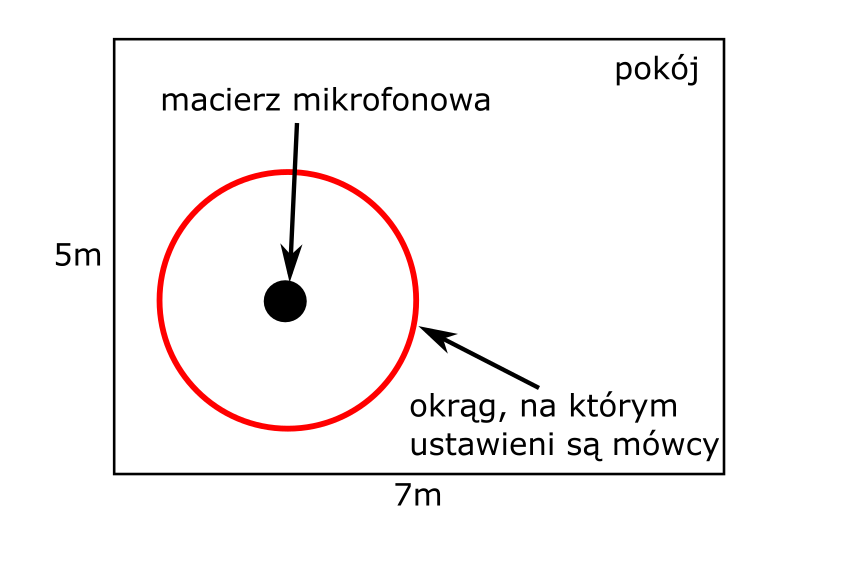
\includegraphics[width=0.4\textwidth]{Images/room.png}
    \caption{Symulowany Pokój}
    \label{fig:room}
\end{figure}

\begin{figure}[h!]
    \centering
    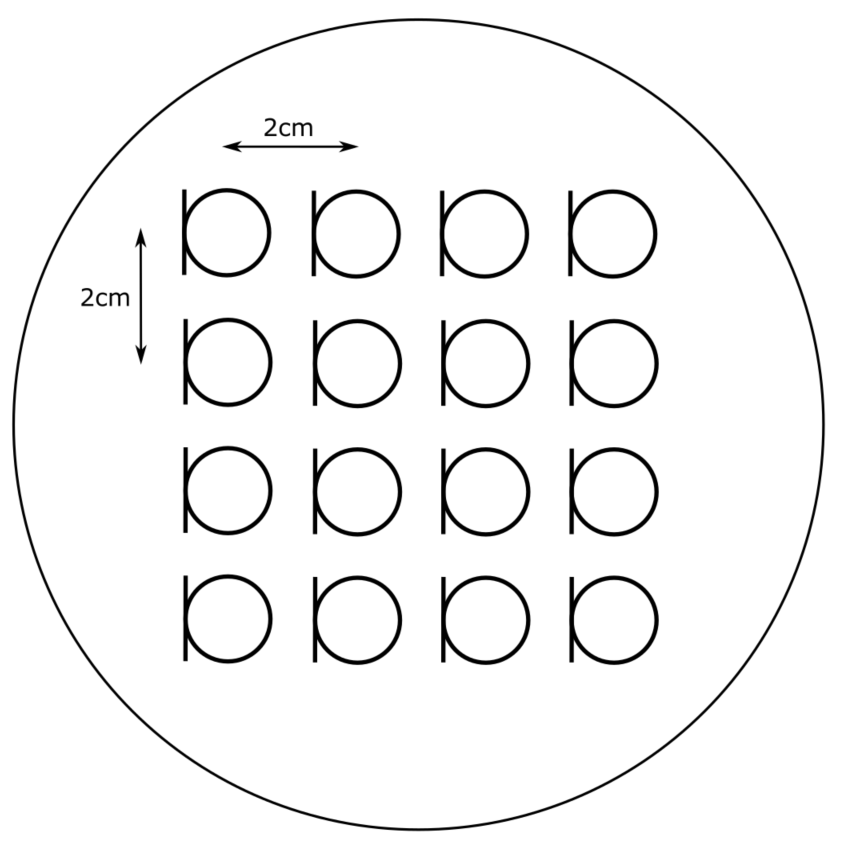
\includegraphics[width=0.4\textwidth]{Images/microphone.png}
    \caption{Macierz Mikrofonowa}
    \label{fig:microphone}
\end{figure}

\noindent Jako zakłócenie do usunięcia wybrano biały szum. Jego macierz PSD może być zapisana jako macierz diagonalna z wartościami 1 na przekątnej $\bm{\Phi}_{\mathrm{n}} = \bm{\mathrm{diag}}(1)$.

\noindent W sekcjach poniżej kolejno opisywane są wykonywane testy i doświadczenia.

\section{Charakterystyka kierunkowa filtra LCMV}

Poniżej przedstawiono wykresy charakterystyki kierunkowej dla filtra LCMV o następujących parametrach:

\begin{itemize}
    \item $\theta_{0}=30^{\circ}, \,
    \theta_{1}=120^{\circ}, \,
    \theta_{2}=300^{\circ}$
    \item $G(\theta_{0})=4, \,
    G(\theta_{1})=2, \,
    G(\theta_{2})=1$
\end{itemize}
\noindent dla częstotliwości 100Hz, 500Hz i 2kHz.

\begin{figure}[h!]
    \centering
    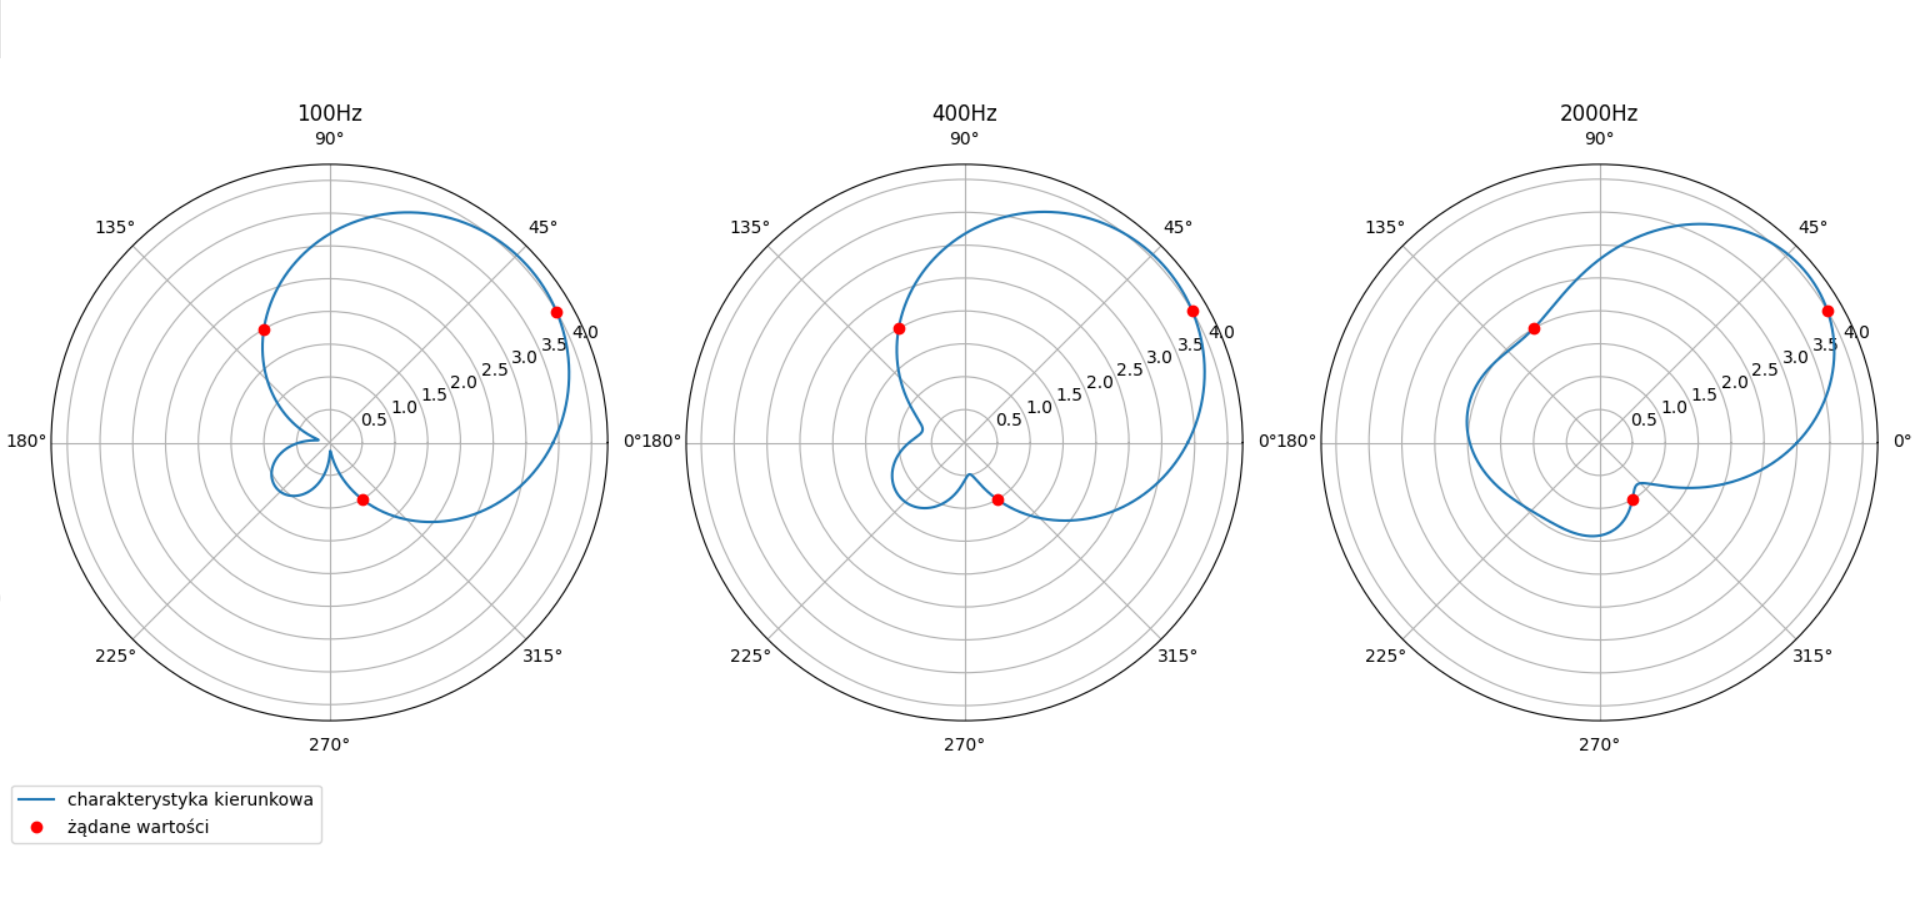
\includegraphics[width=\textwidth]{Images/directivity0.02m.png}
    \caption{Charakterystyka kierunkowa dla $\Delta d = 2cm$}
    \label{fig:directivity0.02}
\end{figure}

\noindent Załączony obrazek \ref{fig:directivity0.02} pokazuje, że filtr prawidłowo generuje wymuszenia w określonych kierunkach. Właściwości usuwania tła akustycznego zostaną sprawdzone w kolejnych sekcjach.

\noindent Zgodnie z teorią przedstawioną w \cite{mccowan2001} wraz ze wzrostem stosunku $\dfrac{\Delta d}{\lambda}$, gdzie $\lambda$ to długość fali, rośnie kierunkowość filtru. Prowadzi to do sytuacji, w której maksima są bardzo wąskie i wartość charakterystyki kierunkowej silnie fluktuuje w dziedzinie kątów. Nieznaczny błąd estymacji kierunku nadchodzenia fali może więc prowadzić do fatalnych skutków. Zjawisko pojawiania się dużej liczby minimów i maksimów nazywane jest aliasingiem przestrzennym. Zachodzi dla $\Delta d > \dfrac{\lambda}{2}$. Przy założonej prędkości dzwięku dla częstotliwości $f = 4kHz$ granica aliasingu przestrzennego wystąpi dla $\Delta d \approx 4cm $. Dlatego właśnie zdecydowano się wybrać bezpieczną odległość między mikrofonami $\Delta d = 2cm$.

\noindent Warte pokazania są wykresy takich samych filtrów jeśli mikrofony byłyby oddalone od siebie odpowiednio o $\Delta d = 20cm$ i $\Delta d = 2m$:

\begin{figure}[h!]
    \centering
    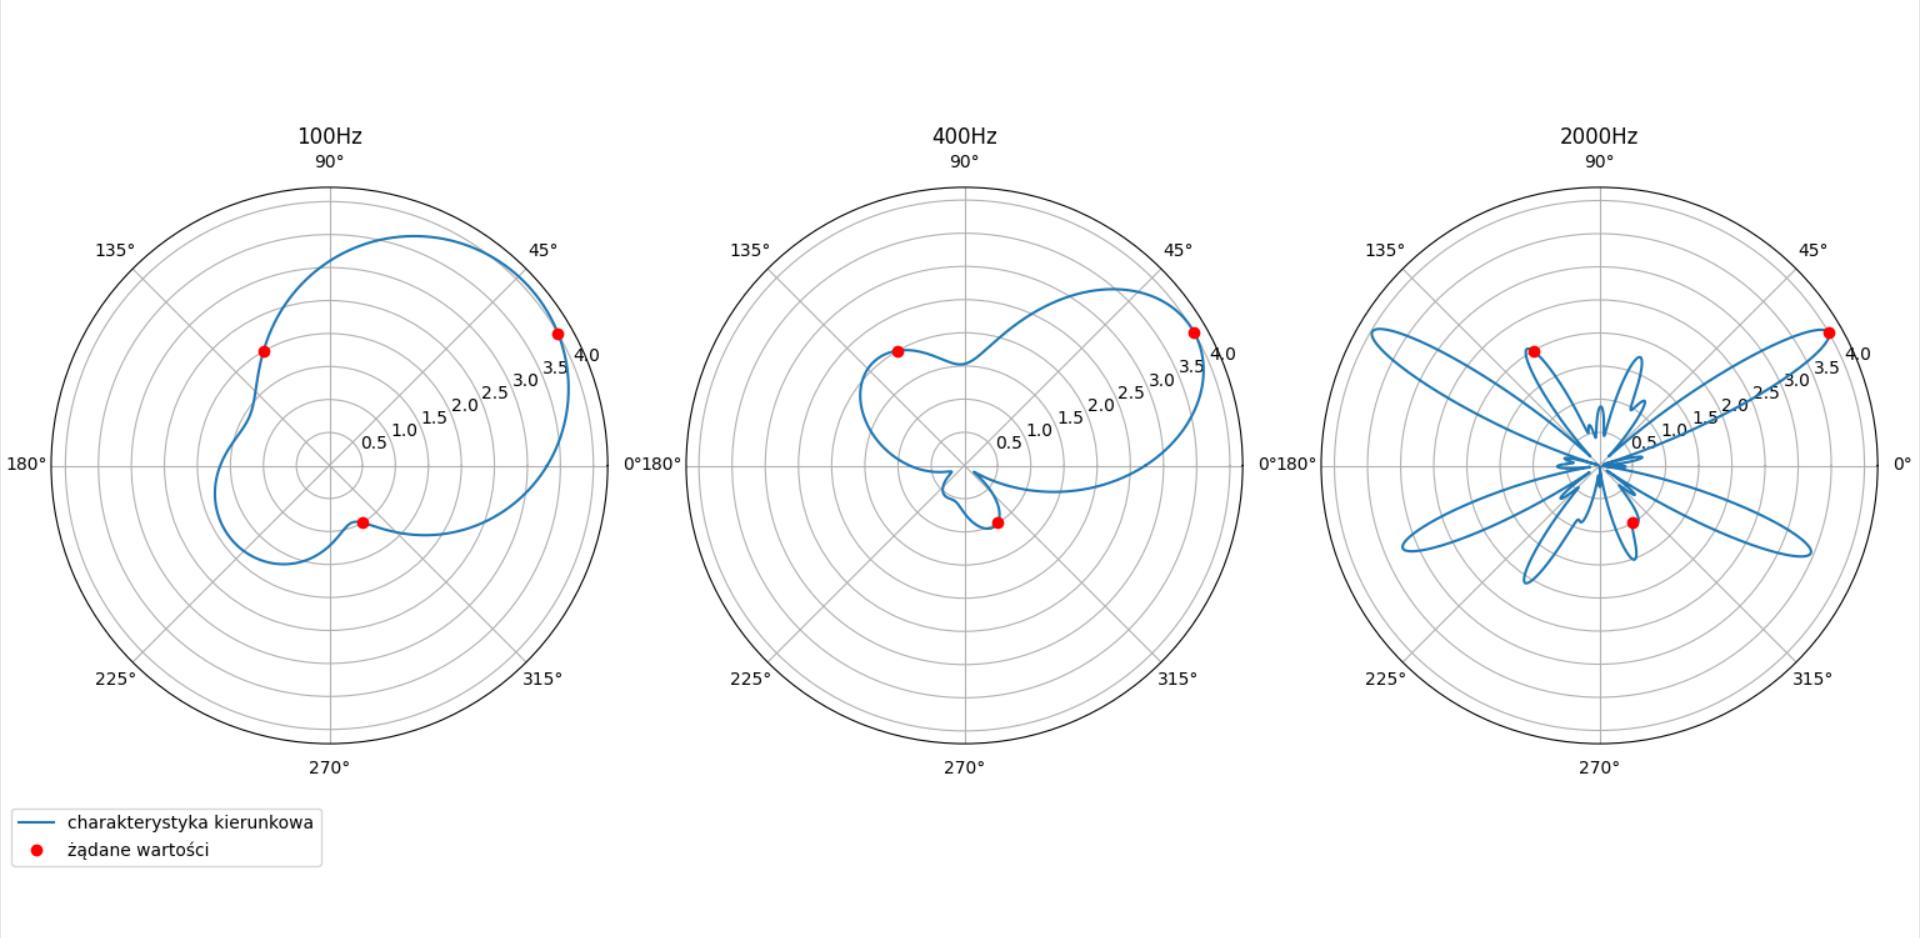
\includegraphics[width=\textwidth]{Images/directivity0.2m.png}
    \caption{Charakterystyka kierunkowa dla $\Delta d = 20cm$}
    \label{fig:directivity0.2}
\end{figure}

\begin{figure}[h!]
    \centering
    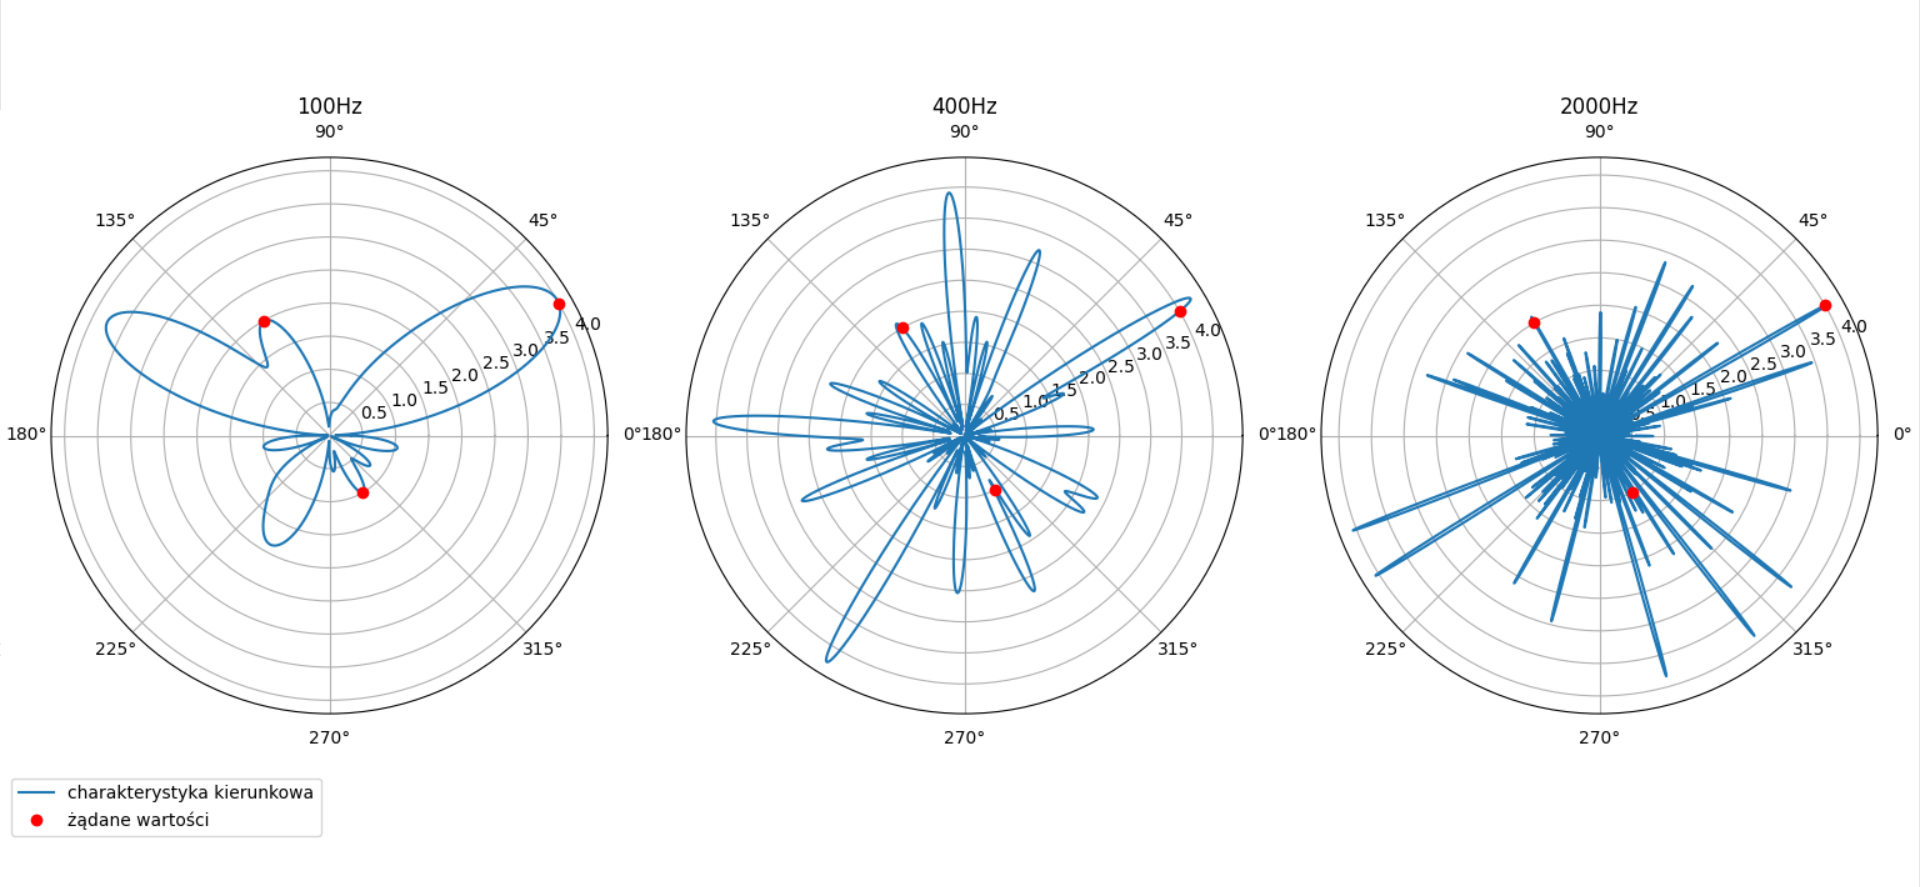
\includegraphics[width=\textwidth]{Images/directivity2m.png}
    \caption{Charakterystyka kierunkowa dla $\Delta d = 2m$}
    \label{fig:directivity2}
\end{figure}

\newpage

\section{Ewaluacja algorytmu MUSIC}

\noindent W celu sprawdzenia działania zaproponowanego algorytmu MUSIC sprawdzone są różne warianty rozłożenia mówców:

\begin{itemize}
    \item Jeden mówca usytuowany na kącie $\theta_{0} = 78^{\circ}$
    \item Trzech mówców usytuowanych na kątach $\theta_{0} = 78^{\circ}, \, \theta_{1} = 192^{\circ}, \, \theta_{2} = 301^{\circ}$
\end{itemize}
\noindent Wszystkie powyższe scenariusze będą powtórzone dla następjących konfiguracji wartości stosunku sygnału do szumu i obecności pogłosu:

\begin{itemize}
    \item $\mathrm{SNR}=10\mathrm{dB}$ 
    \item $\mathrm{SNR}=-10\mathrm{dB}$
    \item $\mathrm{SNR}=10\mathrm{dB}, \, $ sygnał z pogłosem
\end{itemize}

\noindent Te wartości zostały sprawdzone dla $\Delta d = 2cm$ i $\Delta d = 20cm$ dla porównania. Wygenerowane wykresy przedstawiające znalezione DOA mogą być znalezione w tekście jako załączniki \ref{fig:music_10db_2cm}-\ref{fig:music_10db_20cm_reverb}. Na przedstawionych wykresach po lewej stronie znajduje się efekt działania dla jednego źródła a po prawej dla trzech źródeł.

\begin{figure}[H]
    \centering
    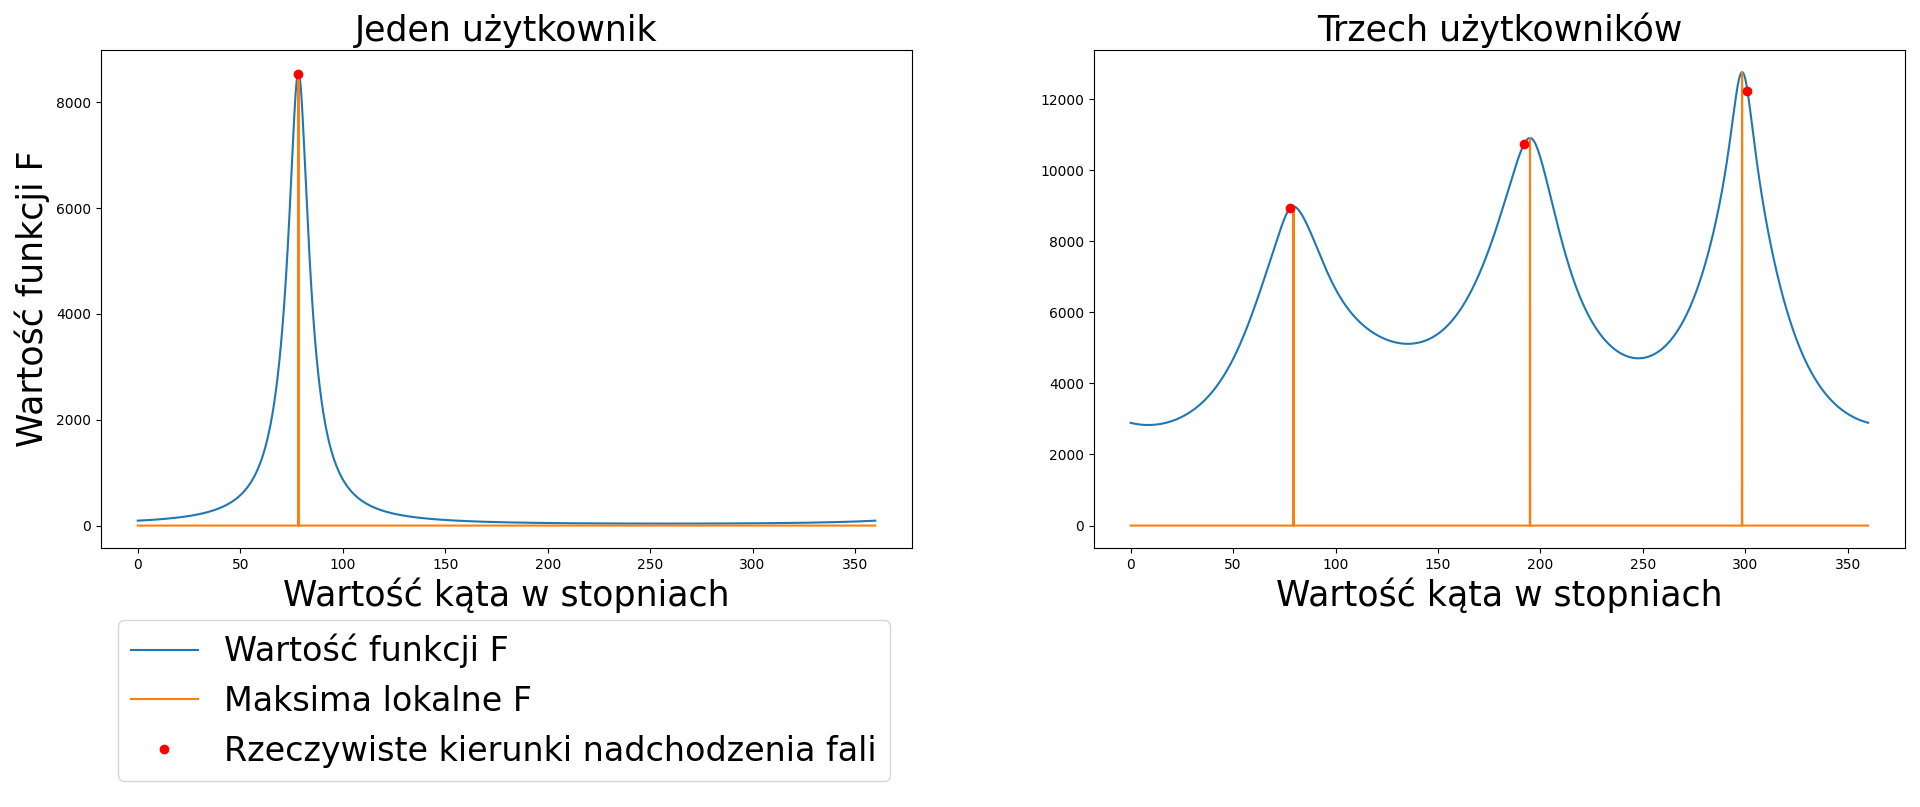
\includegraphics[width=0.85\textwidth]{Images/music_10db.png}
    \caption{$\mathrm{SNR}=10\mathrm{dB}, \, \Delta d = 2cm$}
    \label{fig:music_10db_2cm}
\end{figure}

\begin{figure}[H]
    \centering
    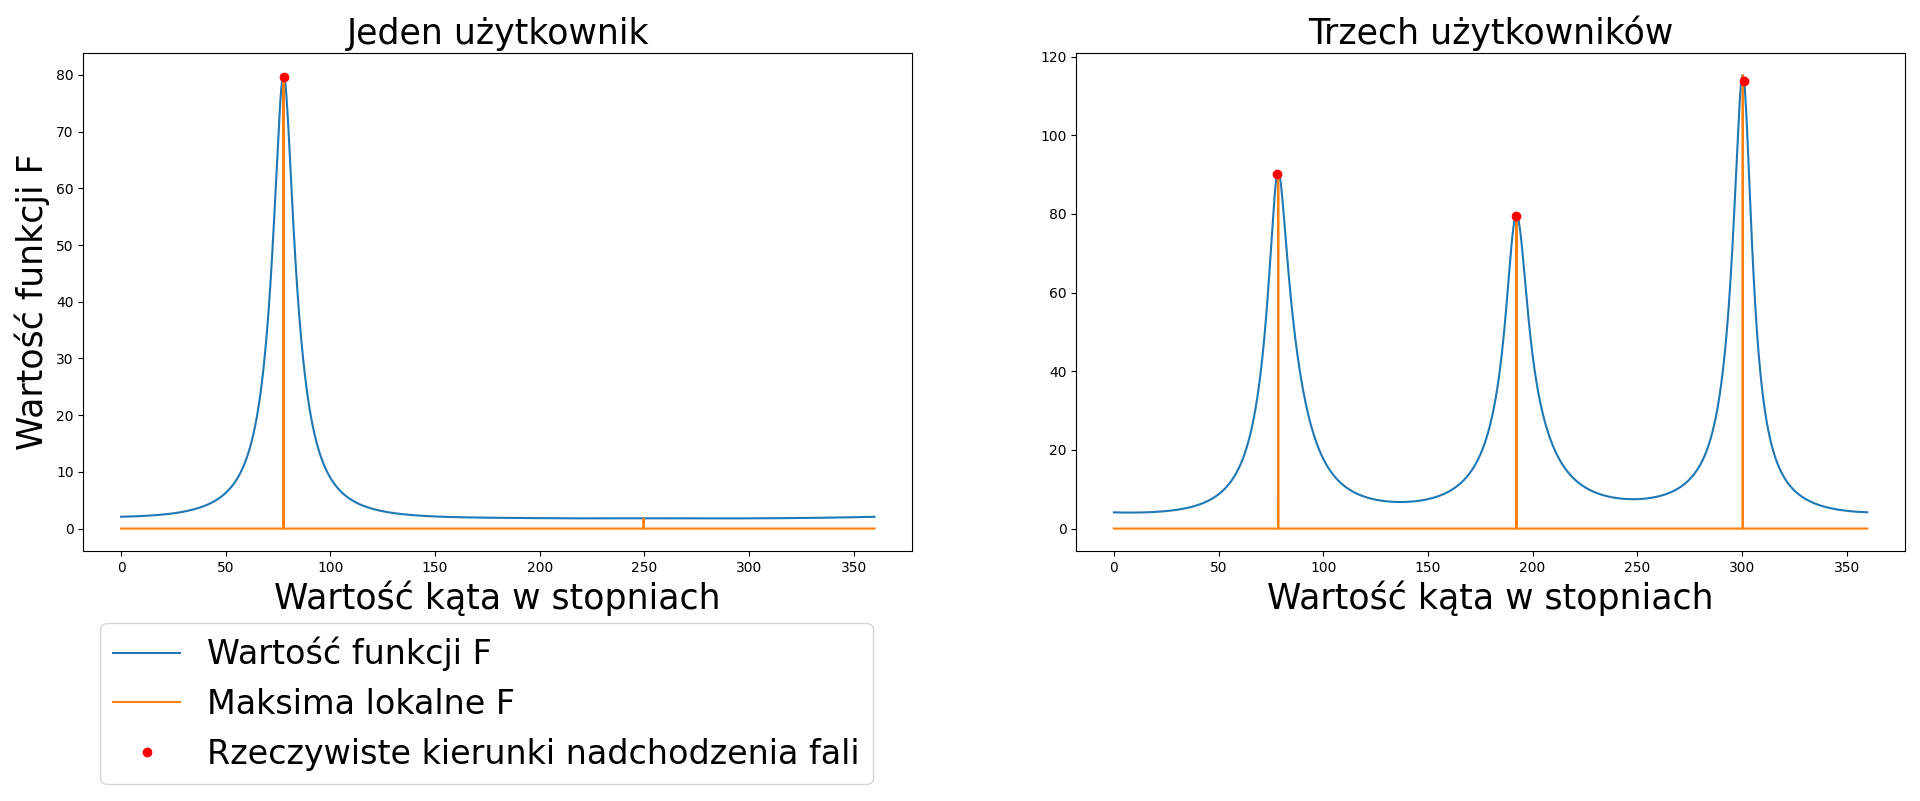
\includegraphics[width=0.85\textwidth]{Images/music_-10db.png}
    \caption{$\mathrm{SNR}=-10\mathrm{dB}, \, \Delta d = 2cm$}
    \label{fig:music_-10db_2cm}
\end{figure}

\begin{figure}[H]
    \centering
    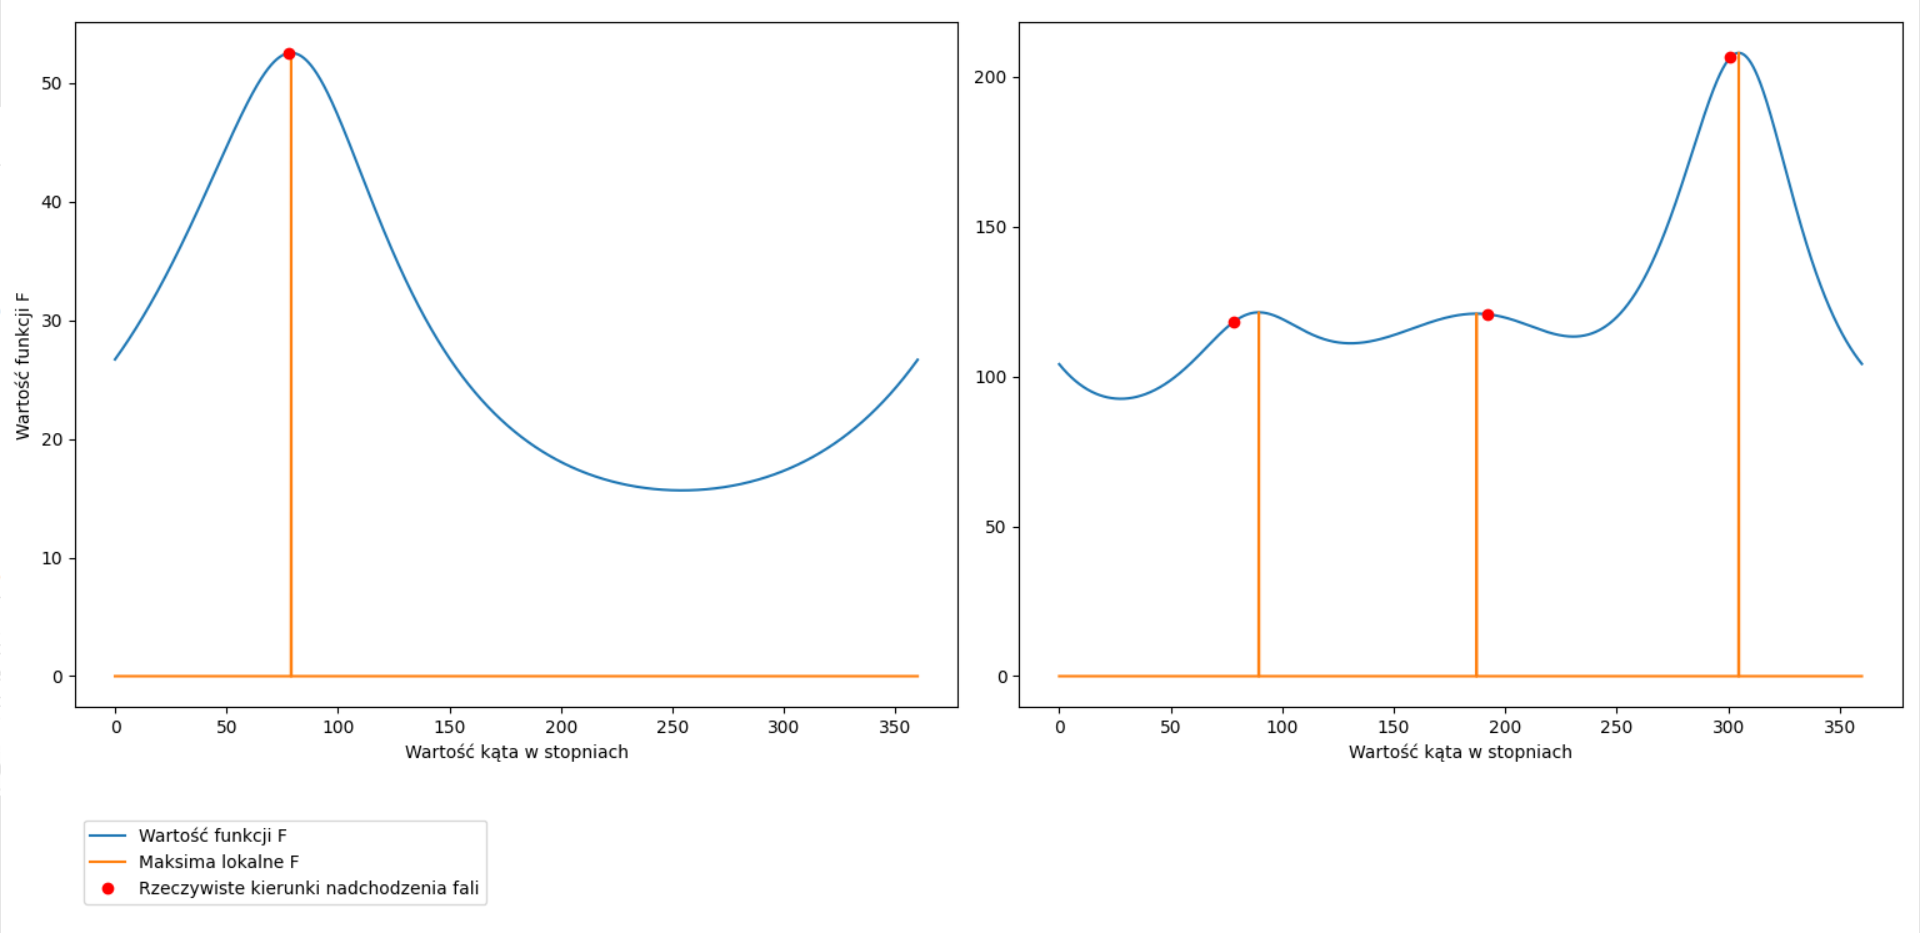
\includegraphics[width=0.85\textwidth]{Images/music_10db_reverb.png}
    \caption{$\mathrm{SNR}=10\mathrm{dB}, \, \Delta d = 2cm$ z pogłosem}
    \label{fig:music_10db_2cm_reverb}
\end{figure}

\begin{figure}[H]
    \centering
    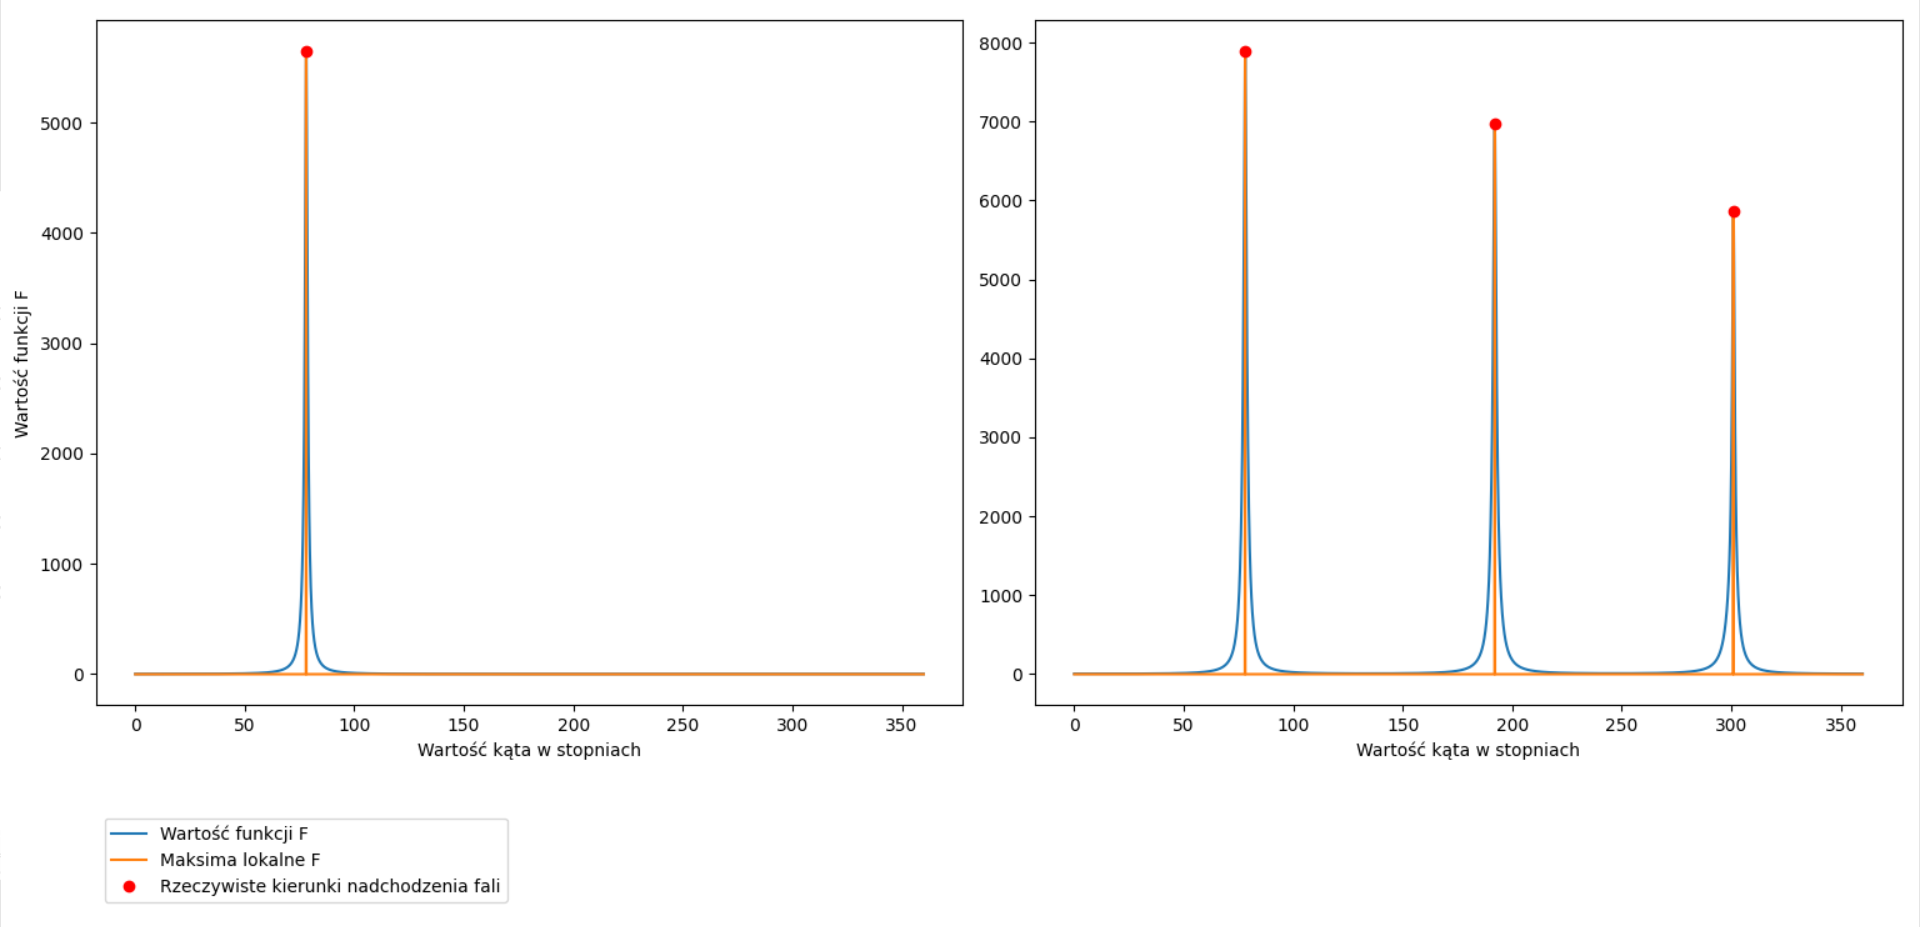
\includegraphics[width=0.85\textwidth]{Images/music_10db_0.2m.png}
    \caption{$\mathrm{SNR}=10\mathrm{dB}, \, \Delta d = 20cm$}
    \label{fig:music_10db_20cm}
\end{figure}

\begin{figure}[H]
    \centering
    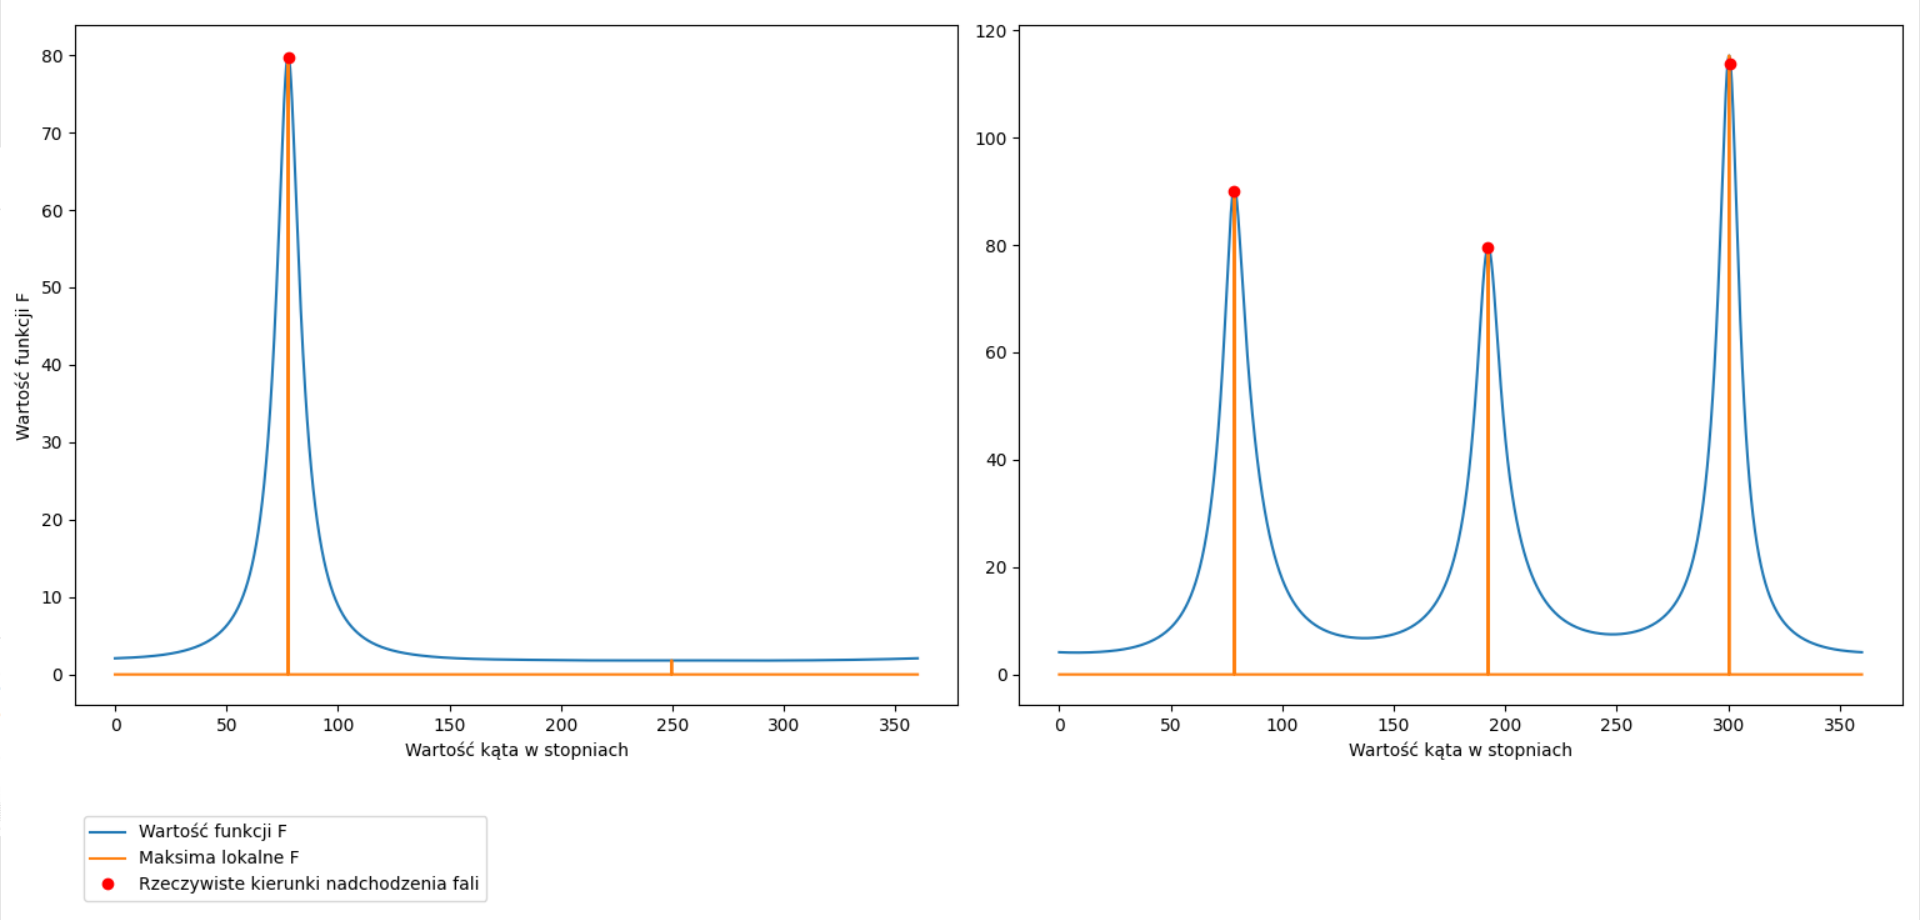
\includegraphics[width=0.85\textwidth]{Images/music_-10db_0.2m.png}
    \caption{$\mathrm{SNR}=-10\mathrm{dB}, \, \Delta d = 20cm$}
    \label{fig:music_-10db_20cm}
\end{figure}

\begin{figure}[H]
    \centering
    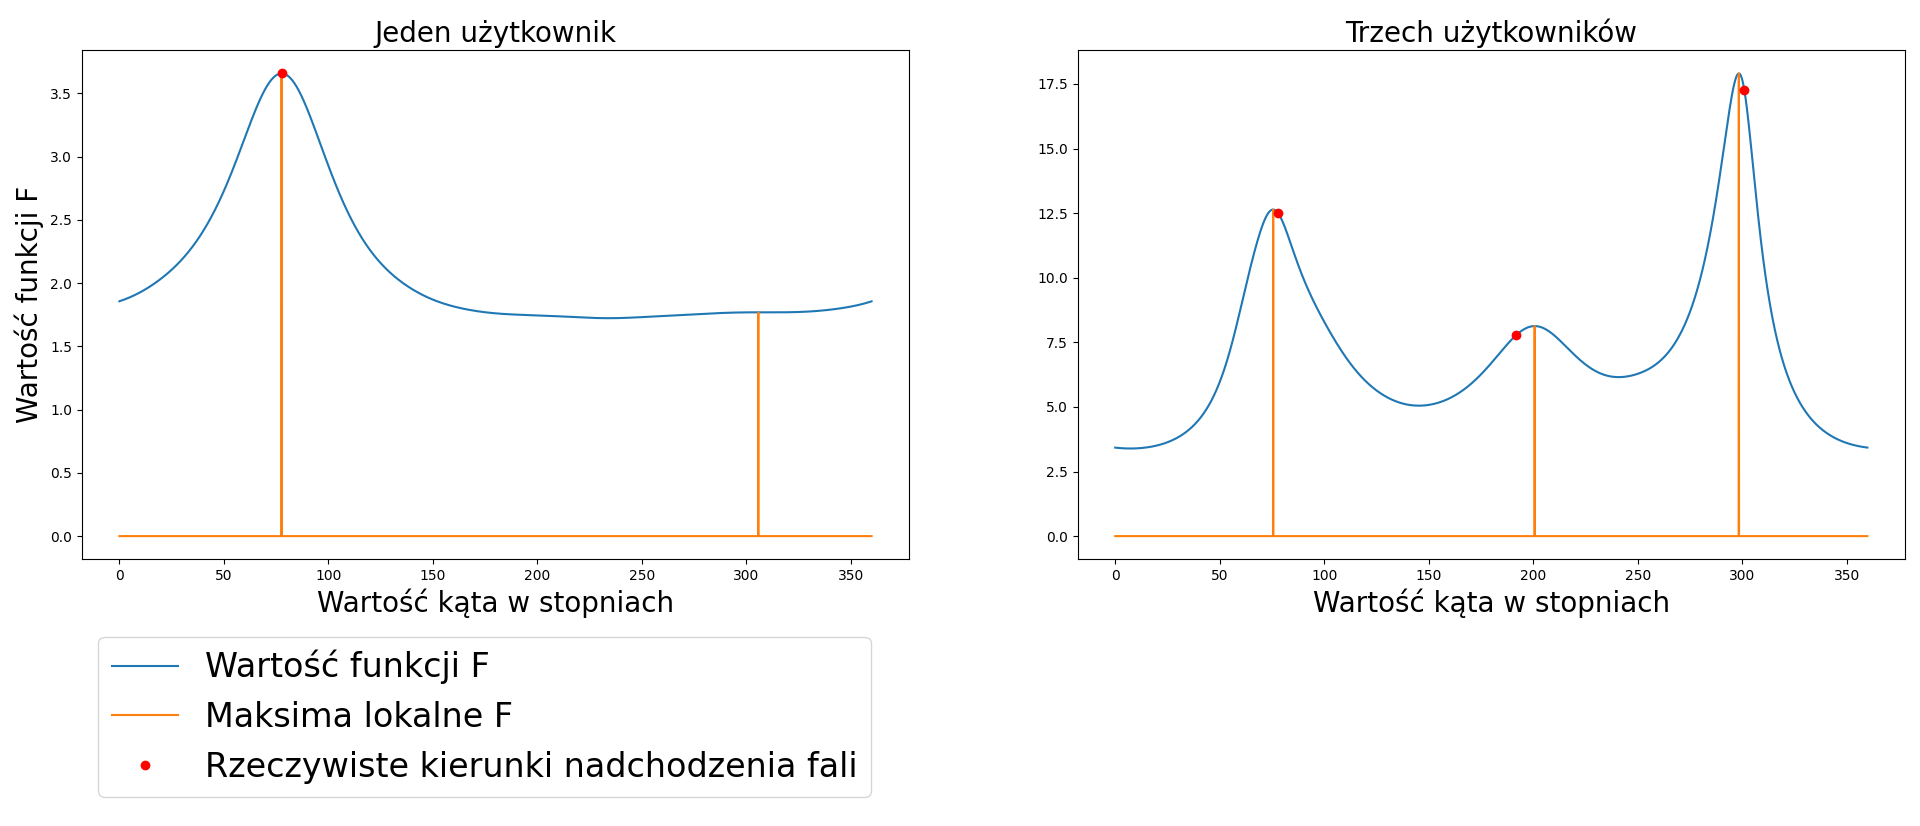
\includegraphics[width=0.85\textwidth]{Images/music_10db_reverb_0.2m.png}
    \caption{$\mathrm{SNR}=10\mathrm{dB}, \, \Delta d = 20cm$ z pogłosem}
    \label{fig:music_10db_20cm_reverb}
\end{figure}

\noindent Wyniki dotyczące wpływu szumu nie zaskakują- algorytm działa mniej dokładnie dla niskiego SNR. To samo dotyczy pogłosu, użyty algorytm nie jest odporny na tego typu zakłócenia. Pojawiające się odbite fale wewnątrz pokoju czynią maksima mniej wybitnymi. Najbardziej interesująca obserwacja zdaniem autora pracy to wpływ odległości między mikrofonami. Większa odległość powoduje większą kierunkowość co przekłada się na dokładniejszą estymację. Dla rozłożenia $\Delta \d = 20cm$ i szumie $\mathrm{SNR}=-10\mathrm{dB}$ udaje się dokładnie wyestomować wszystkie trzy kierunki. Dla tego samego stosunku sygnału do szumu i $\Delta d = 2cm$ algorytm estymuje tylko dwa kierunki i to bardzo niedokładnie. Do dalszych testów wybrano jednak system ze stosunkiem sygnału do szumu na poziomie 10-20dB a mówcy są dość daleko od siebie. Zbytnia kierunkowość powoduje duże problemy z zastosowaniem filtra LCMV i nawet bardzo dokładna estymacja nie rekompensuje tych strat. Doświadczenia empiryczne pokazały, że cały system działa lepiej dla $\Delta d = 2cm$.

\newpage

\section{Testy całego systemy}

Testy całego systemu sprawdzają kilka różnych aspektów projektu inżynierskiego. Są to:

\begin{itemize}
    \item Stosunek sygnału do szumu(SNR)
    \item Ocena działania systemu dla jednego użytkownika
    \item Ocena działania systemu dla wielu użytkowników
    \item Ewaluacja wpływu poruszania się źródła na działanie algorytmu
    \item Sprawdzenie wpływu pogłosu na jakość przetwarzania
    
\end{itemize}
\subsection{SNR}

Obliczenie SNR dla systemu jest obliczane zarówno dla systemu z pojedynczym użytkownikiem jak i z trzema użytkownikami. Aby obliczyć SNR zakłada się, że $\bm{\mathrm{g}} = \{1,..,1\}$ dla każdego indeksu czasowego. Oznacza to wyłączenie AGC. Z włączonym AGC następowałyby zmiany lokalnej amplitudy sygnału uniemożliwiając sensowny pomiar SNR. Wszystkie pomiary SNR podaje się w skali logarytmicznej.

\noindent Zastosowano następującą normę pomiaru poprawy SNR:
\begin{equation}
    \label{delta_SNR}
    \Delta \mathrm{SNR} = \mathrm{SNR}_{\mathrm{output}} - \mathrm{SNR}_{\mathrm{input}}
\end{equation}

\noindent Gdzie SNR na wejściu $\mathrm{SNR}_{\mathrm{input}}$ jest znane a mając do dyspozycji niezaszumiony sygnał referencyjny $x_{\mathrm{ref}}(n)$ i sygnał zaszumiony $x_{\mathrm{noisy}}(n)$ można także obliczyć stosunek sygnału do szumu dla $N$ próbek wyjściowych sygnału jako:

\begin{equation}
    \label{SNR}
    \mathrm{SNR} = 10 \log \sum_{n=1}^{N}\left(
    \dfrac
    {x_{\mathrm{ref}}(n)}
    {x_{\mathrm{ref}}(n)-x_{\mathrm{noisy}}(n)} \right)^{2}
\end{equation}
\noindent Taki pomysł obliczania SNR zaczerpnięto luźno z \cite{Virtanen2006}. Z tą różnicą, że autor tego artykułu obliczał SNR w dziedzinie STFT.

\noindent Uzyskano następujące wyniki:
\begin{itemize}
    \item Pojedynczy użytkownik: $\Delta \mathrm{SNR} \approx 12dB$ 
    \item Trzech użytkowników: $\Delta \mathrm{SNR} \approx 6dB$
\end{itemize}

\noindent Wykresy przedstawiające sygnały przed i po odszumaniu przedstawiono na \ref{fig:snr_boost}

\begin{figure}[H]
    \centering
    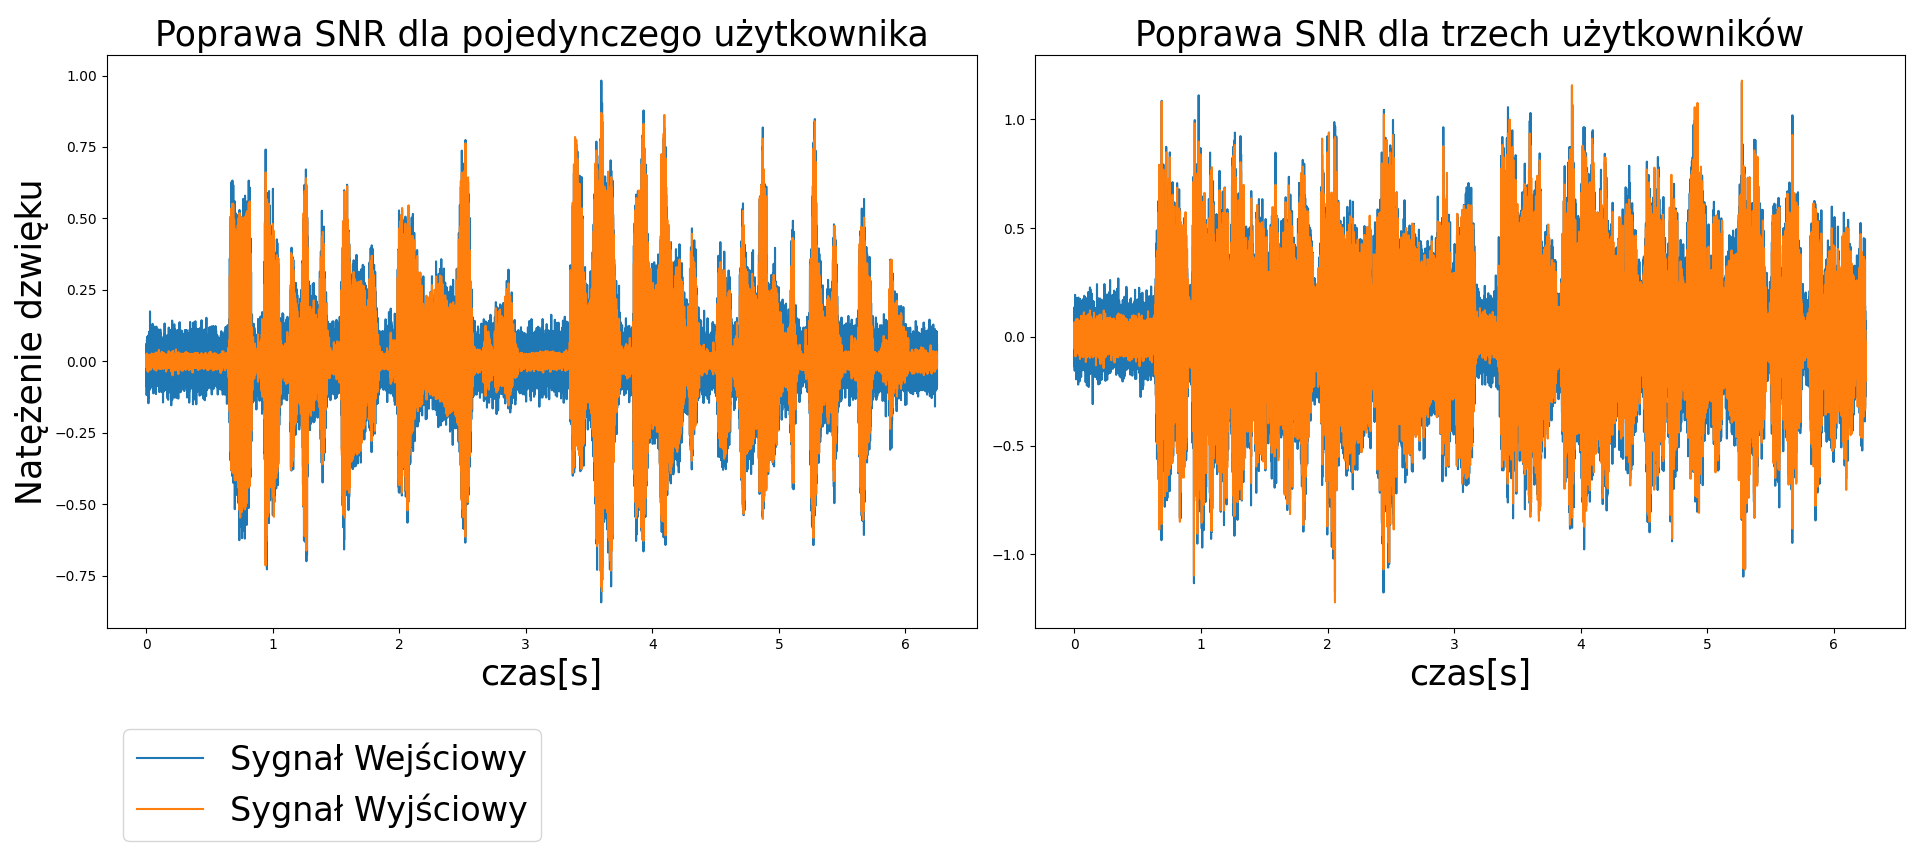
\includegraphics[width=\textwidth]{Images/snr_boost.png}
    \caption{Poprawa SNR}
    \label{fig:snr_boost}
\end{figure}

\subsection{Działanie algorytmu dla pojedynczego użytkownika}

Ocenę algorytmu dla pojedynczego użytkownika przeprowadzono w warunkach gdzie użytkownik jest ustawiony na $\theta_{0}=78^{\circ}$. Nagrany sygnał ma długość 50000 próbek co przekłada się na nieco ponad 6 sekund.
\noindent W celu oceny jakości działania sprawdza się dwa warianty zmian sygnału w czasie:
\begin{itemize}
    \item Dziesięciokrotny wykładniczy wzrost amplitudy w czasie trwania sygnału
    \item Dziesięciokrotny wykładniczy spadek amplitudy w czasie trwania sygnału
\end{itemize}

\noindent W obu przypadkach początkowy SNR wynosi 10dB. Wyniki eksperymentu przedstawiono na wykresach \ref{fig:single_user_increasing} i \ref{fig:single_user_decreasing}

\begin{figure}[H]
    \centering
    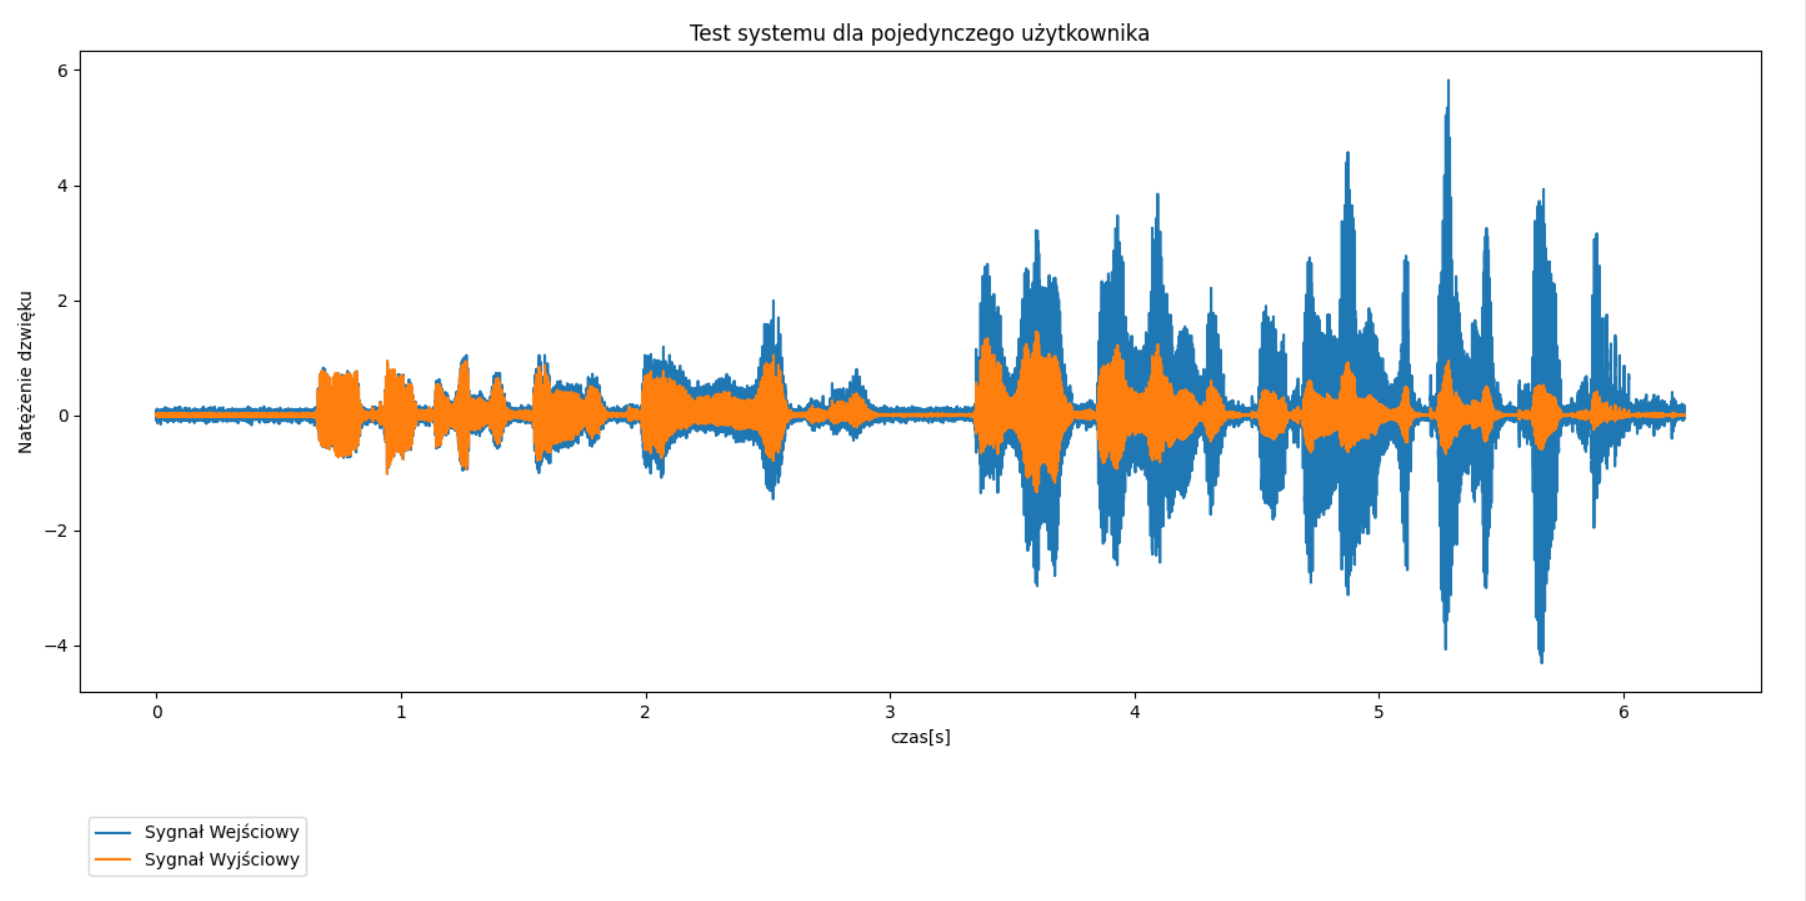
\includegraphics[width=\textwidth]{Images/single_user_increasing.png}
    \caption{Wzrost amplitudy sygnału dla pojedynczego użytkownika}
    \label{fig:single_user_increasing}
\end{figure}

\begin{figure}[H]
    \centering
    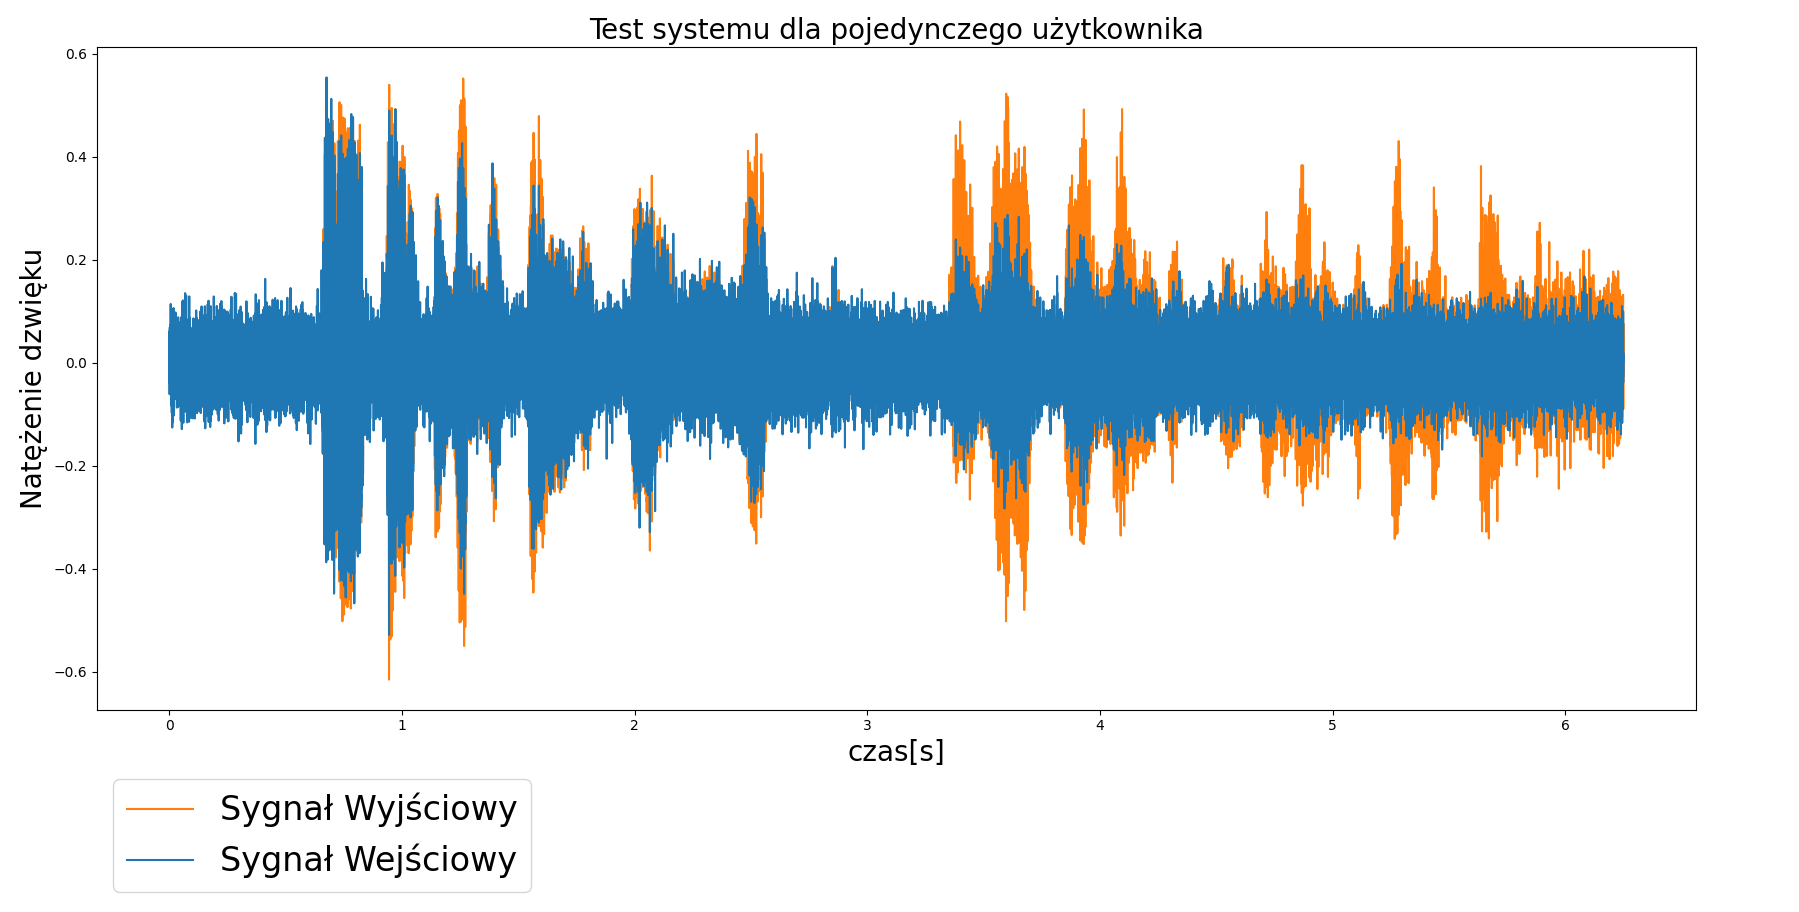
\includegraphics[width=\textwidth]{Images/single_user_decreasing.png}
    \caption{Spadek amplitudy sygnału dla pojedynczego użytkownika}
    \label{fig:single_user_decreasing}
\end{figure}

\noindent Wyniki wymagają krótkiego komentarza. Widoczne jest, że w obu przypadkach mimo, że amplituda sygnału wejściowego silnie zmienia się w czasie, sygnał wyjściowy utrzymuje względnie stały poziom obwiedni. Szczególnie interesujący jest fakt, że w przypadku słabnącego sygnały wejściowego wzmocnienie sygnału powoduje jego wyjście ponad poziom szumu.

\subsection{Działanie algorytmu dla wielu użytkowników}

W przypadku wielu użytkowników nie jest tak łatwo zaprezentować działanie algorytmu za pomocą wykresu wyjściowego. W celu oceny działania algorytmu konieczne będzie obejrzenie zależności wewnętrzych pomiędzy sygnałami $\Phi_{\mathrm{LT}}$, $G'$, $\widehat{G}$. Zmiany parametrów zostaną pokazane zarówno w funkcji czasu jak i w funkcji kąta w pojedynczej ramce. Dla przejrzystości we wszystkich testowanych przypadkach będzie to ta sama ramka.

\noindent Scenariusz testu jest następujący. Natężenie dźwięku pochodzącego od pierwszych dwóch mówców(mężczyźni) jest podobne podczas gdy natężenie trzeciej osoby(kobieta) jest celowo podbite 2 razy. Celem jest wygenerowanie dzwięku, w którym poziom głośności mówców zostanie wyrównany. SNR w tym teście wynosi 20dB aby słabe źródła nie znalazły się zupełnie pod szumem.

\noindent Na wykresach \ref{fig:multi_user}-\ref{fig:multi_user_params_in_angle} przedstawiono wyniki. Przebieg czasowy jest o tyle interesujący, że wyraźnie po momentach ciszy i na początku następuje podbicie sygnału. Dzieje się tak, ponieważ algorytm ustawia dużą głośność dla cichych źródeł i gdy zwiększają one swoją głośność stopiowo ją dostosowuje. Skutkuje to pewnym czasem ustalania się docelowej wartości.

\noindent Na wykresie \ref{fig:multi_user_params_in_time} widoczne jest, że funkcja głośności ma dla źródła głośniejszego wartość mniejszą niż dla cichszego co jest celem działania algorytmu.

\noindent Wykres \ref{fig:multi_user_params_in_angle} świetnie przedstawia ideę zastosowania okien w dziedzinie kątów. Skutkuje to powstaniem charakterystycznych "górek". Mały błąd estymacji nie spowoduje drastycznej zmiany w systemie. Warto też zauważyć górki występujące poza kierunkami nadchodzenia fali. Biorą się one z grubszych błędów estymacji.

\begin{figure}[h!]
    \centering
    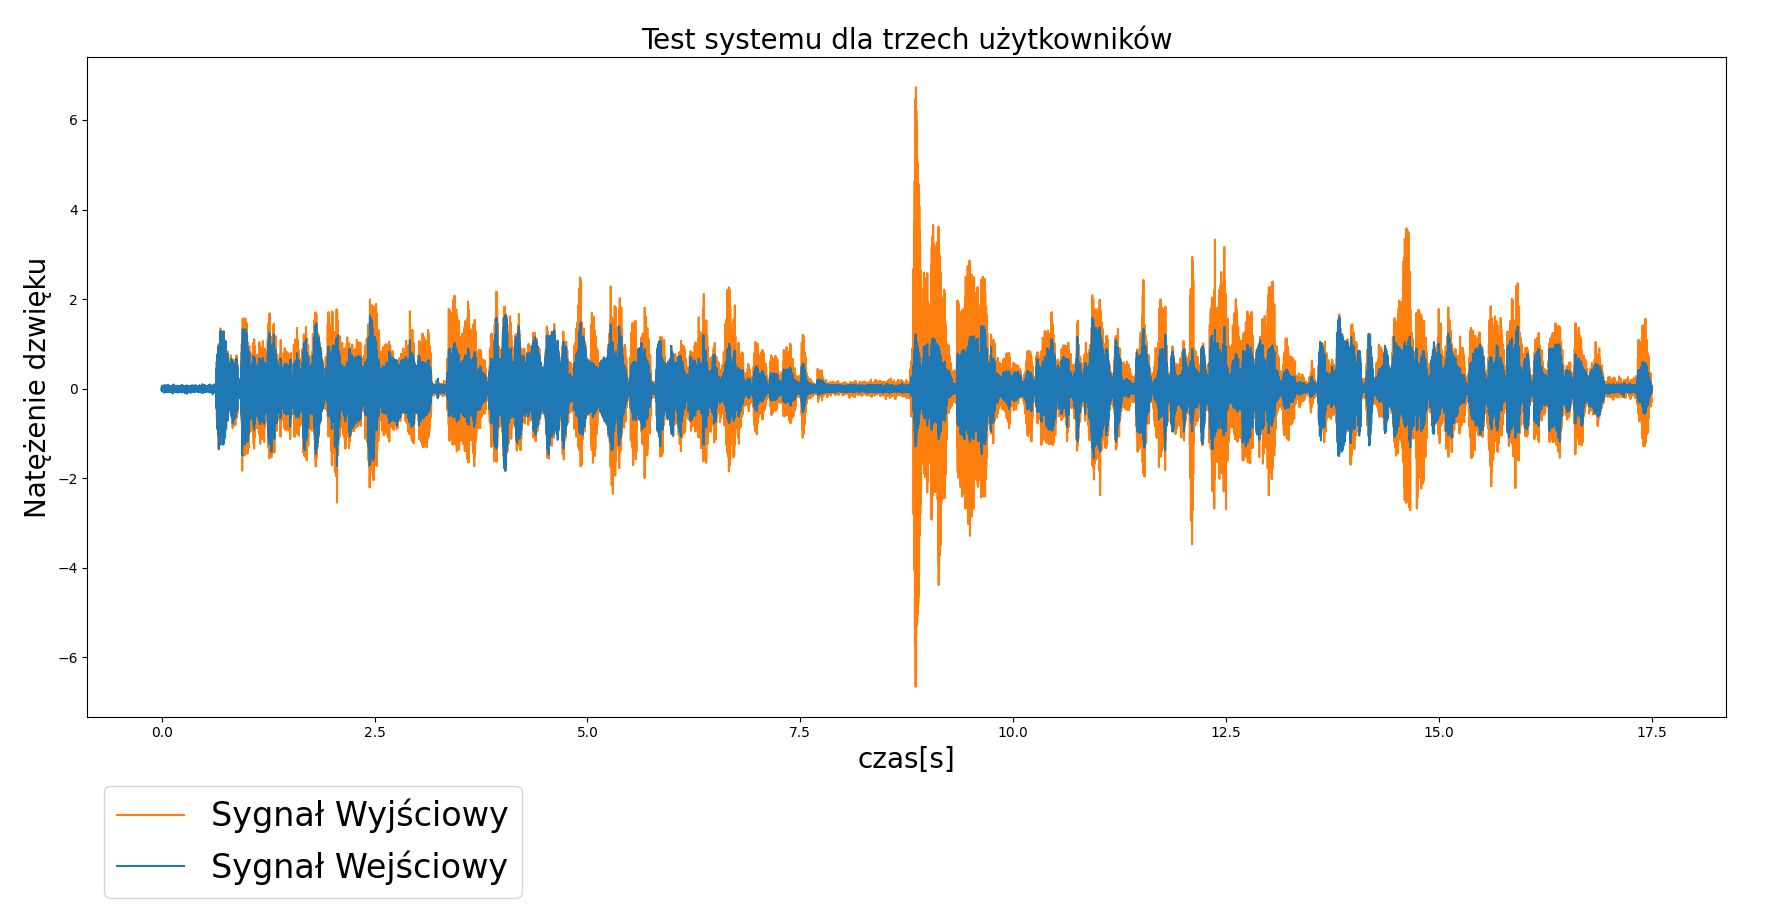
\includegraphics[width=\textwidth]{Images/multi_user.png}
    \caption{Przebieg czasowy dla trzech mówców}
    \label{fig:multi_user}
\end{figure}

\begin{figure}[h!]
    \centering
    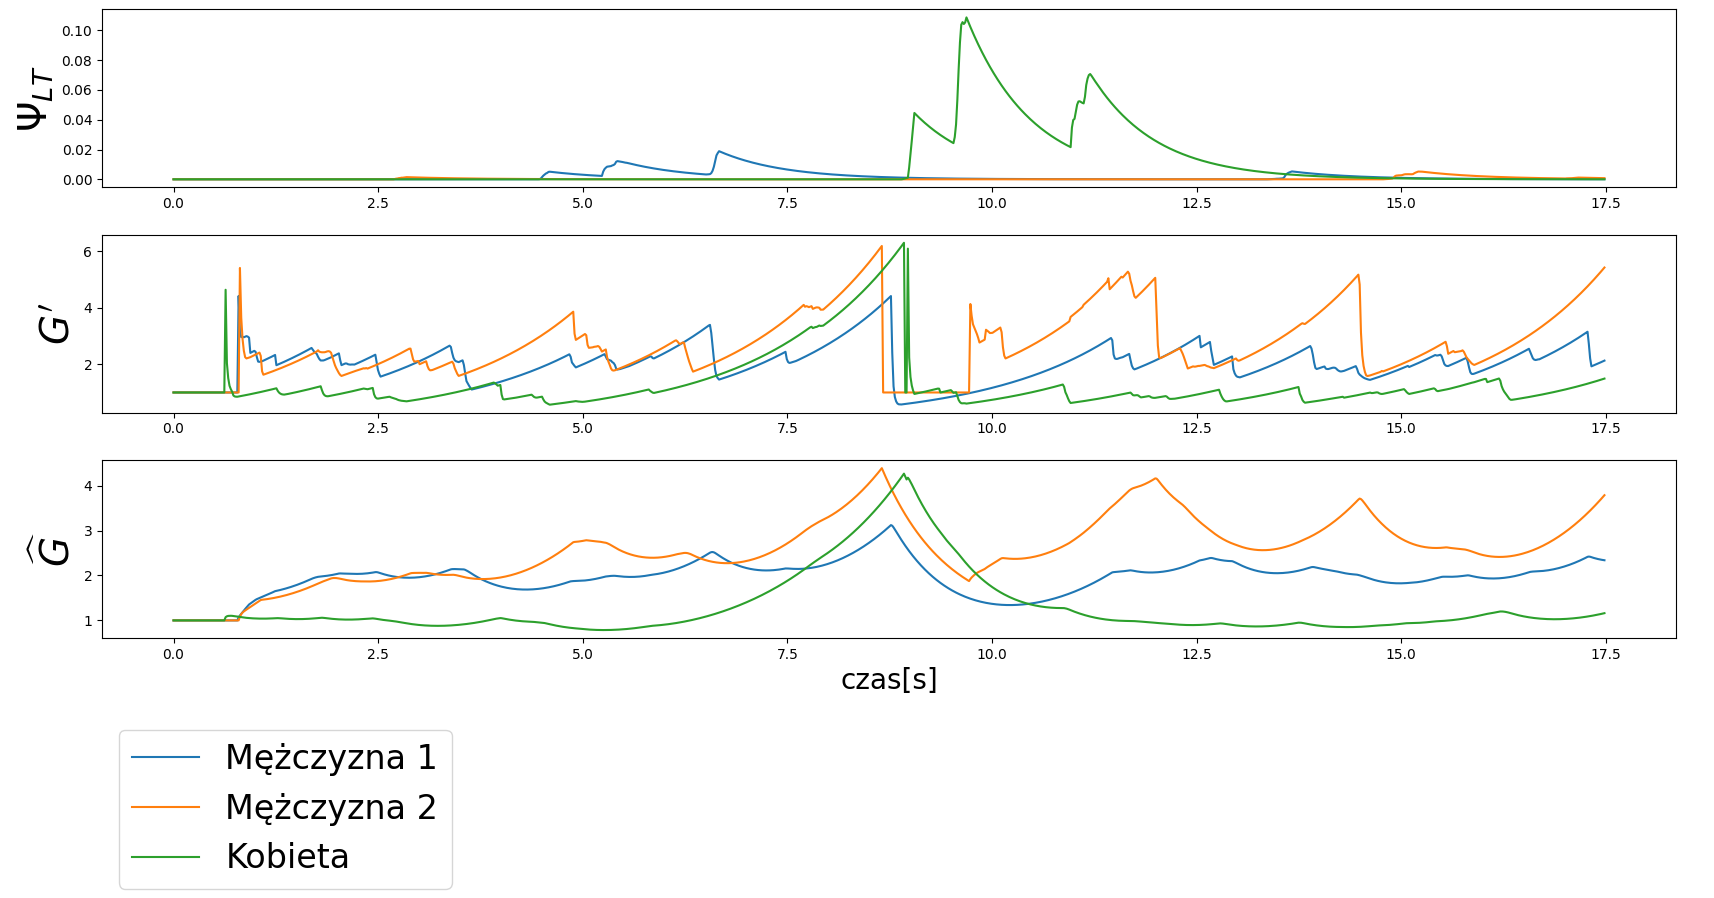
\includegraphics[width=\textwidth]{Images/multi_user_params_in_time.png}
    \caption{Przebieg czasowy wybranych parametrów dla trzech mówców dla kierunków nadchodzenia fali}
    \label{fig:multi_user_params_in_time}
\end{figure}

\begin{figure}[h!]
    \centering
    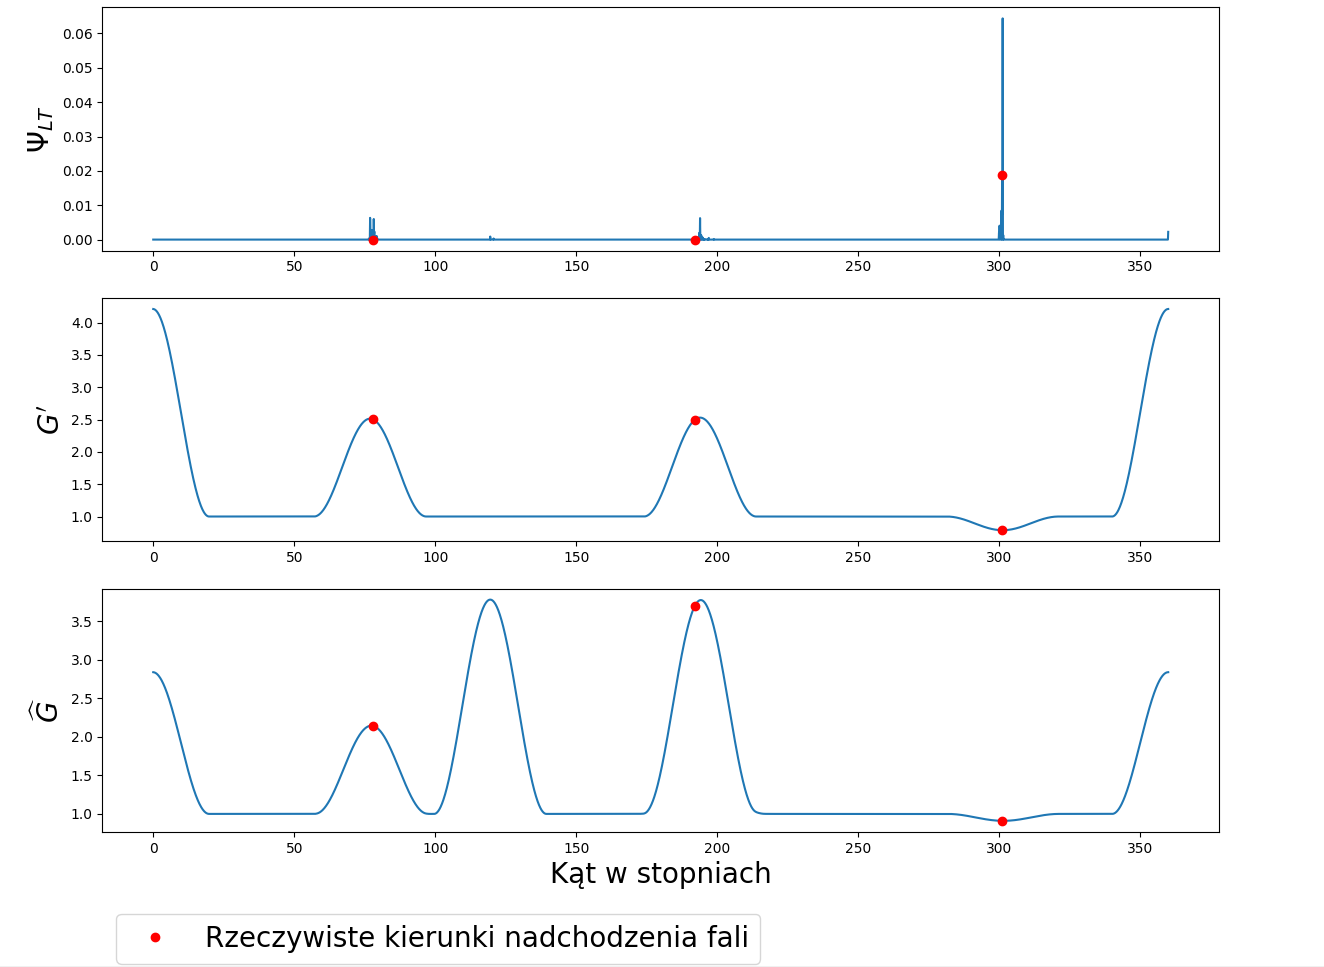
\includegraphics[width=\textwidth]{Images/multi_user_params_in_angle.png}
    \caption{Wybrane parametry jako funkcja kąta w pojedynczej ramce}
    \label{fig:multi_user_params_in_angle}
\end{figure}

\noindent Te same trzy wykresy przedstawiono w wariancie bez estymacji DOA(\ref{fig:multi_user_no_doa}-\ref{fig:multi_user_no_doa_params_in_angle}). Oznacza to, że do algorytmu na twardo podawane są prawdziwie kierunki nadchodzenia fali. Widocznym jest, że zanikają "górki" dla kierunków poza DOA.

\begin{figure}[h!]
    \centering
    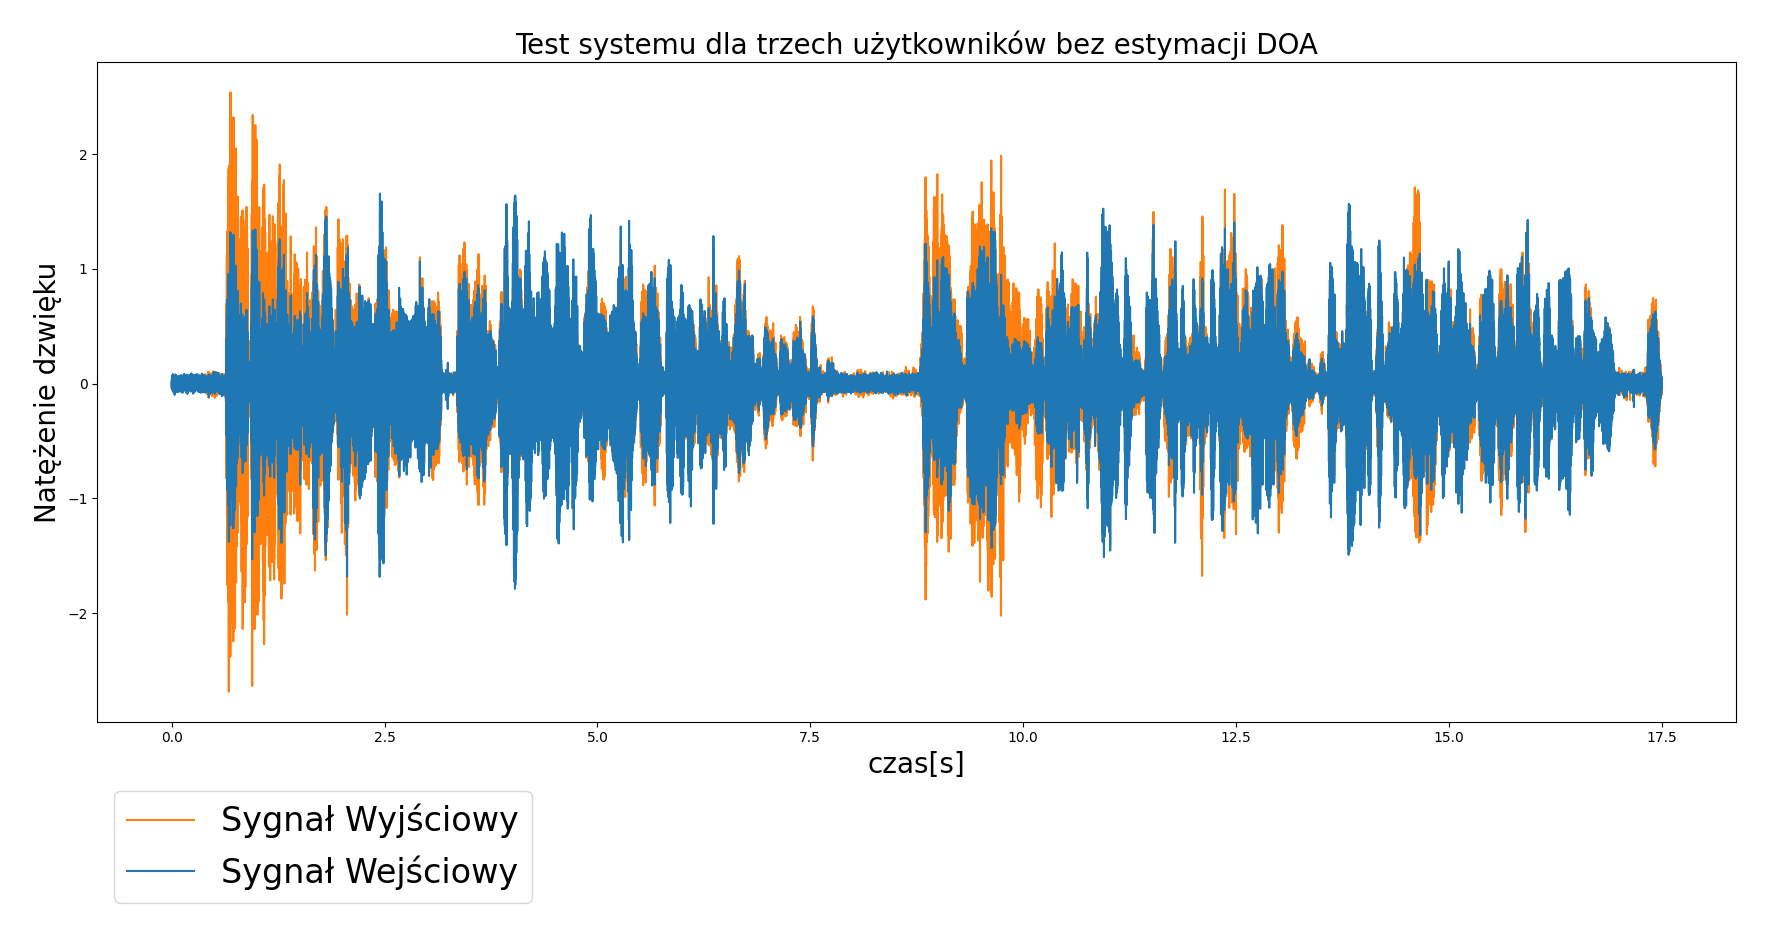
\includegraphics[width=\textwidth]{Images/multi_user_no_doa.png}
    \caption{Przebieg czasowy dla trzech mówców bez estymacji DOA}
    \label{fig:multi_user_no_doa}
\end{figure}

\begin{figure}[h!]
    \centering
    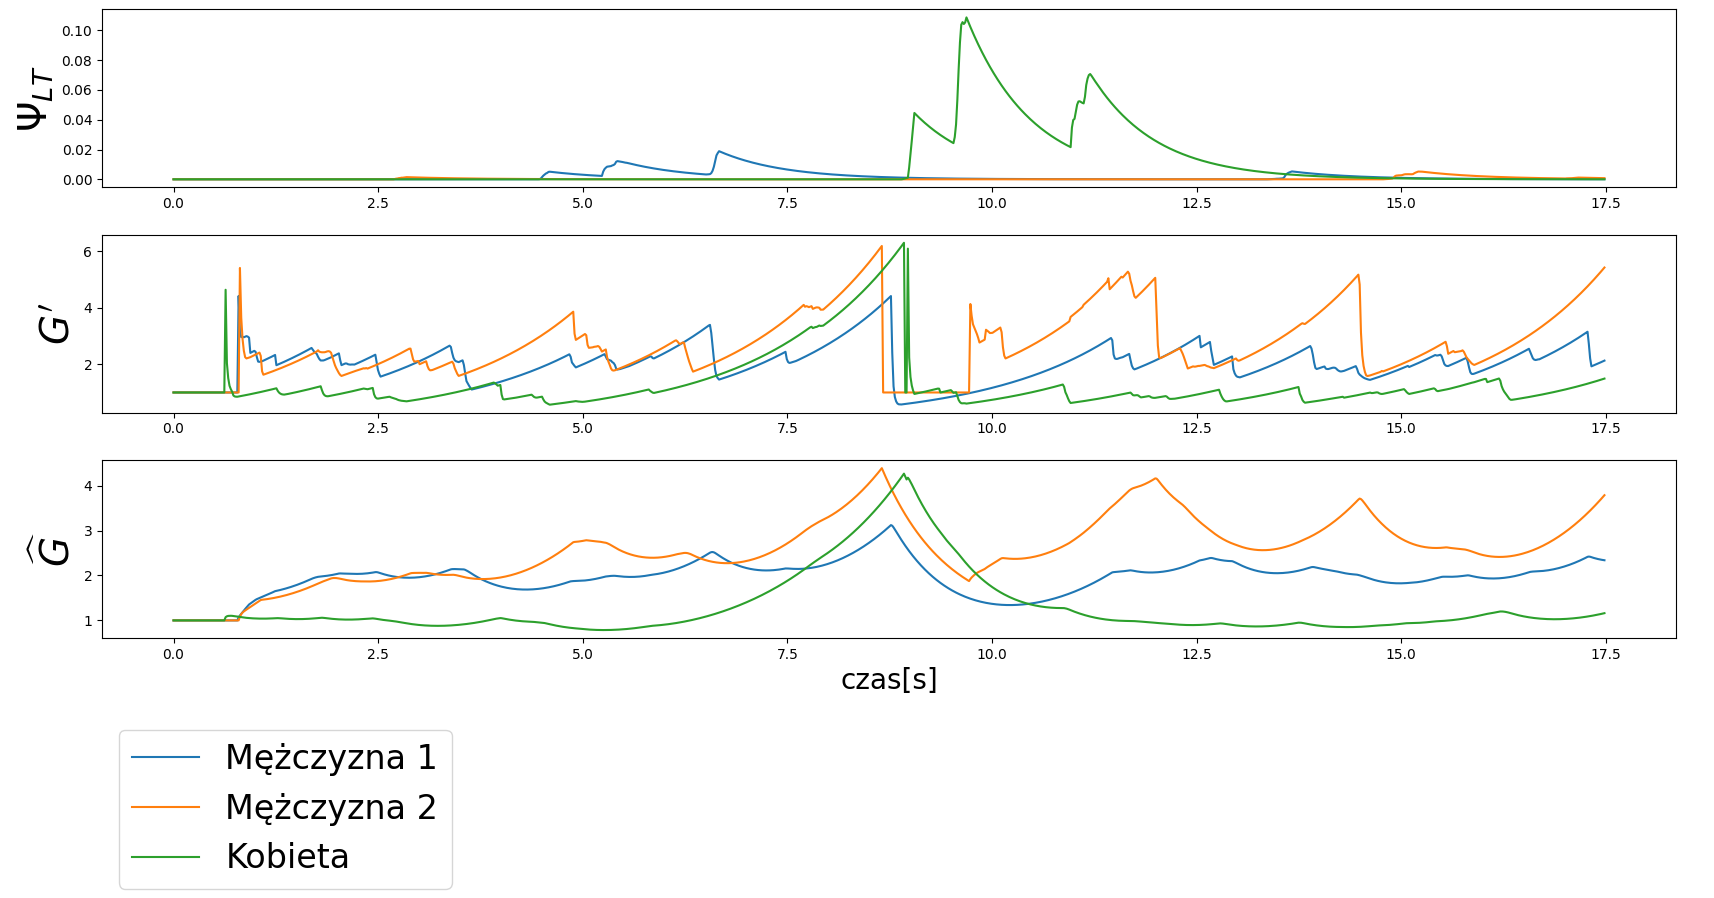
\includegraphics[width=\textwidth]{Images/multi_user_params_in_time.png}
    \caption{Przebieg czasowy wybranych parametrów dla trzech mówców dla kierunków nadchodzenia fali bez estymacji DOA}
    \label{fig:multi_user_no_doa_params_in_time}
\end{figure}

\begin{figure}[h!]
    \centering
    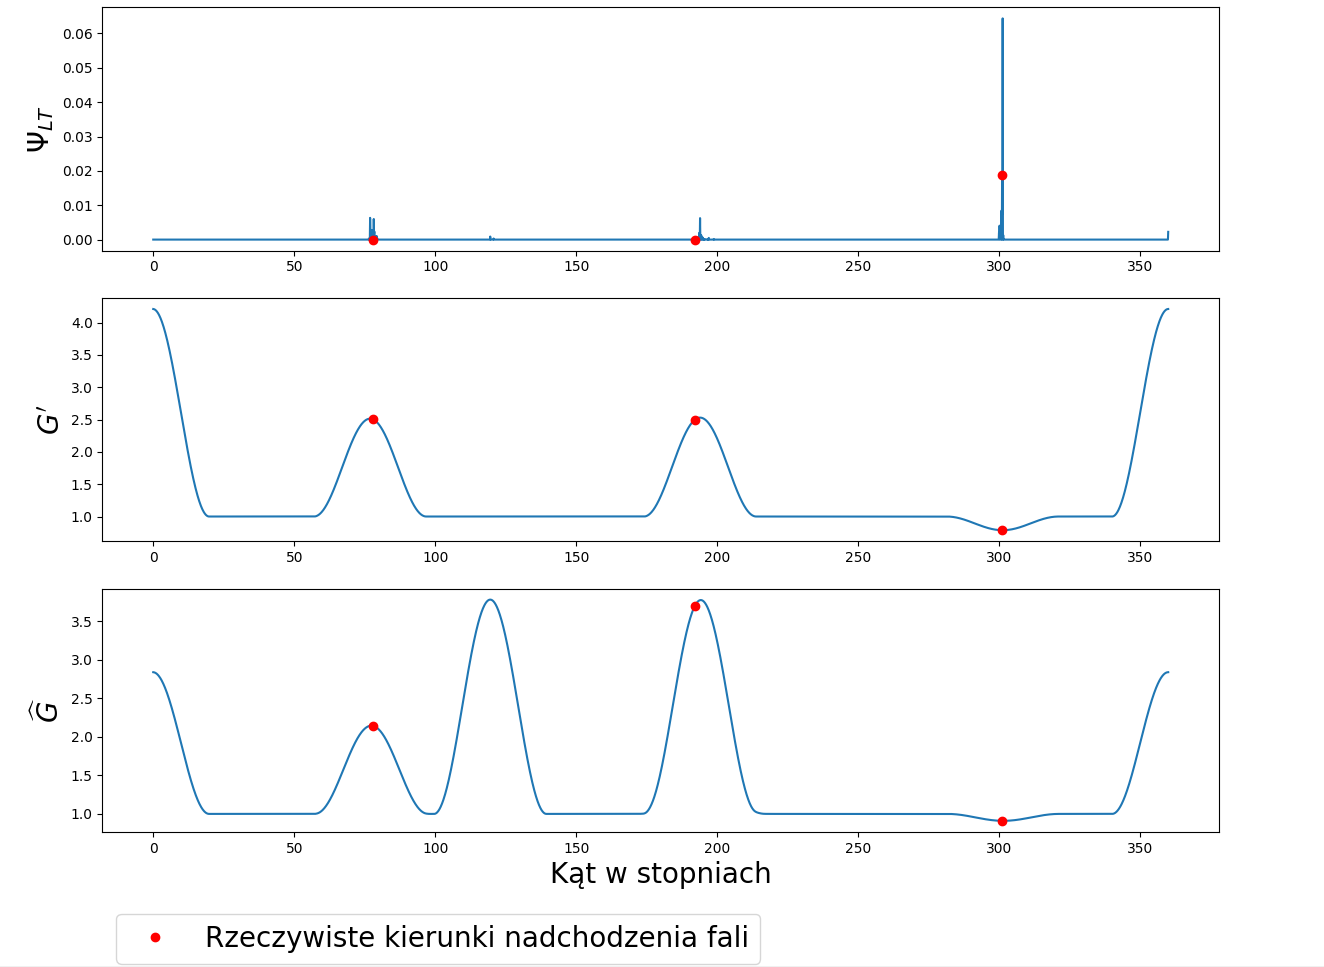
\includegraphics[width=\textwidth]{Images/multi_user_params_in_angle.png}
    \caption{Wybrane parametry jako funkcja kąta w pojedynczej ramce dla przypadku bez estymacji DOA}
    \label{fig:multi_user_no_doa_params_in_angle}
\end{figure}

\subsection{Działanie algorytmu w przypadku ruchu mówcy}

Ten test ma za zadanie sprawdzić czy system AGC będzie działał gdy mówca zacznie się poruszać z niewielką prędkością kątową. Wszystkie parametry są takie jak dla poprzednich testów ale podczas trwania sygnału jeden z mówców- Mężczyzna 1 przemieści się z $78^{\circ} $ na $ 99^{\circ}$.
Na wykresach \ref{fig:moving}-\ref{fig:moving_params_in_angle} pokazano to samo co dla poprzednich przypadków.

\begin{figure}[h!]
    \centering
    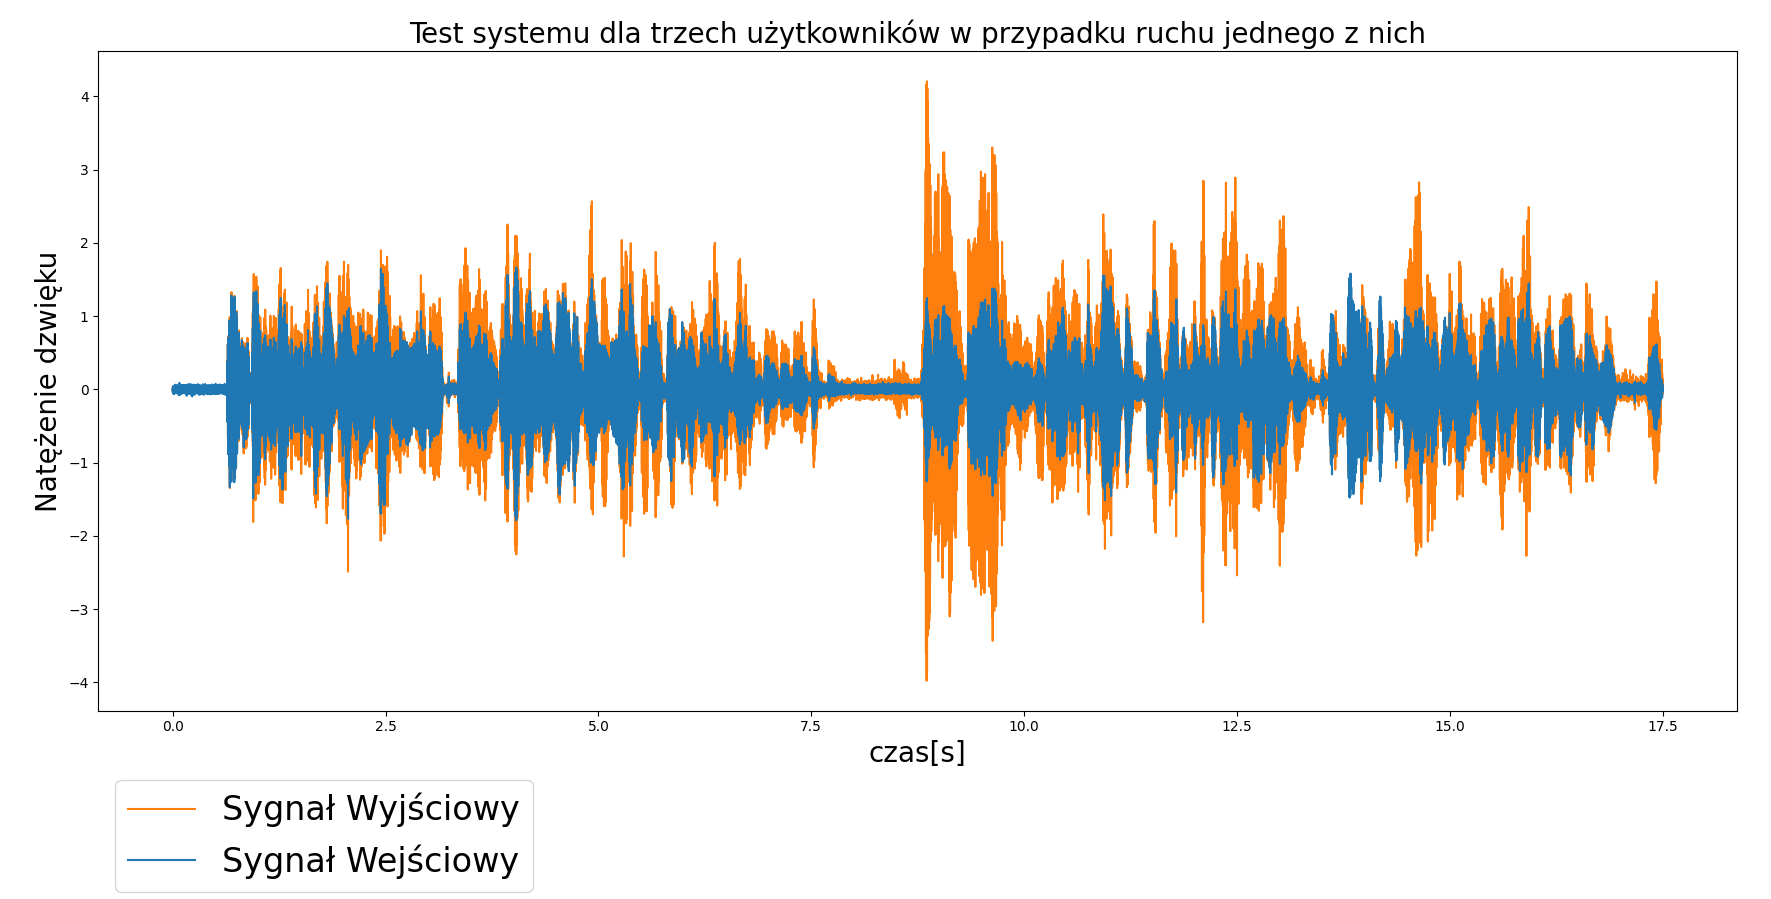
\includegraphics[width=\textwidth]{Images/moving.png}
    \caption{Przebieg czasowy dla trzech mówców w przypadku ruchu jednego z nich}
    \label{fig:moving}
\end{figure}

\begin{figure}[h!]
    \centering
    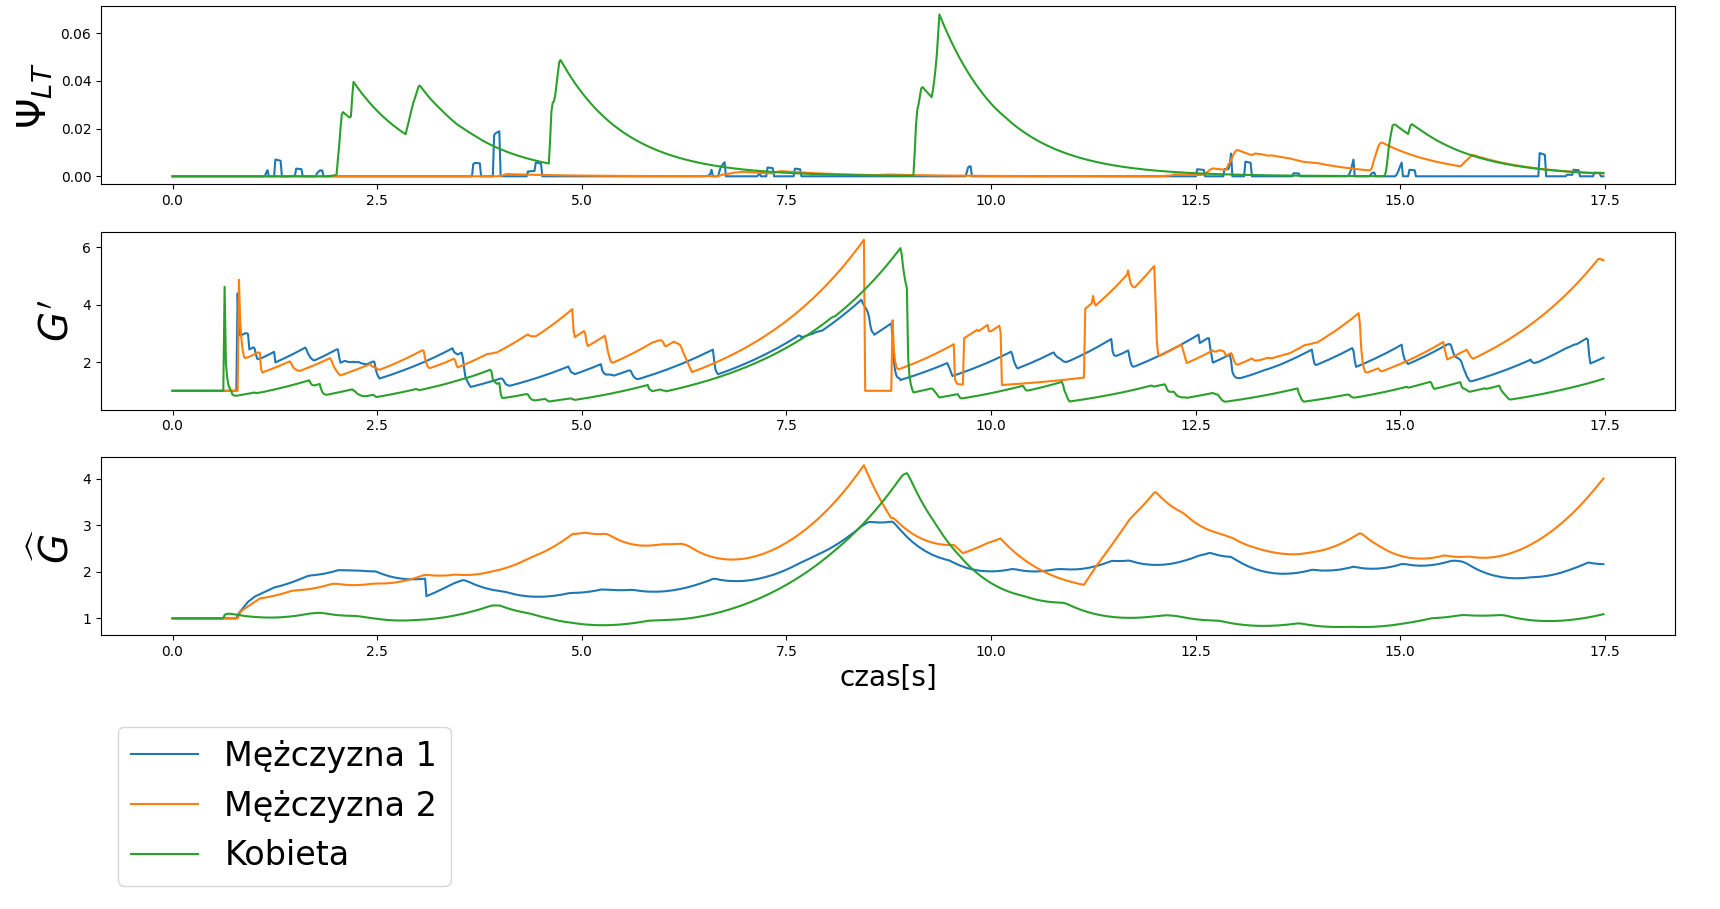
\includegraphics[width=\textwidth]{Images/moving_params_in_time.png}
    \caption{Przebieg czasowy wybranych parametrów dla trzech mówców dla kierunków nadchodzenia fali w przypadku ruchu jednego z nich}
    \label{fig:moving_params_in_time}
\end{figure}

\begin{figure}[h!]
    \centering
    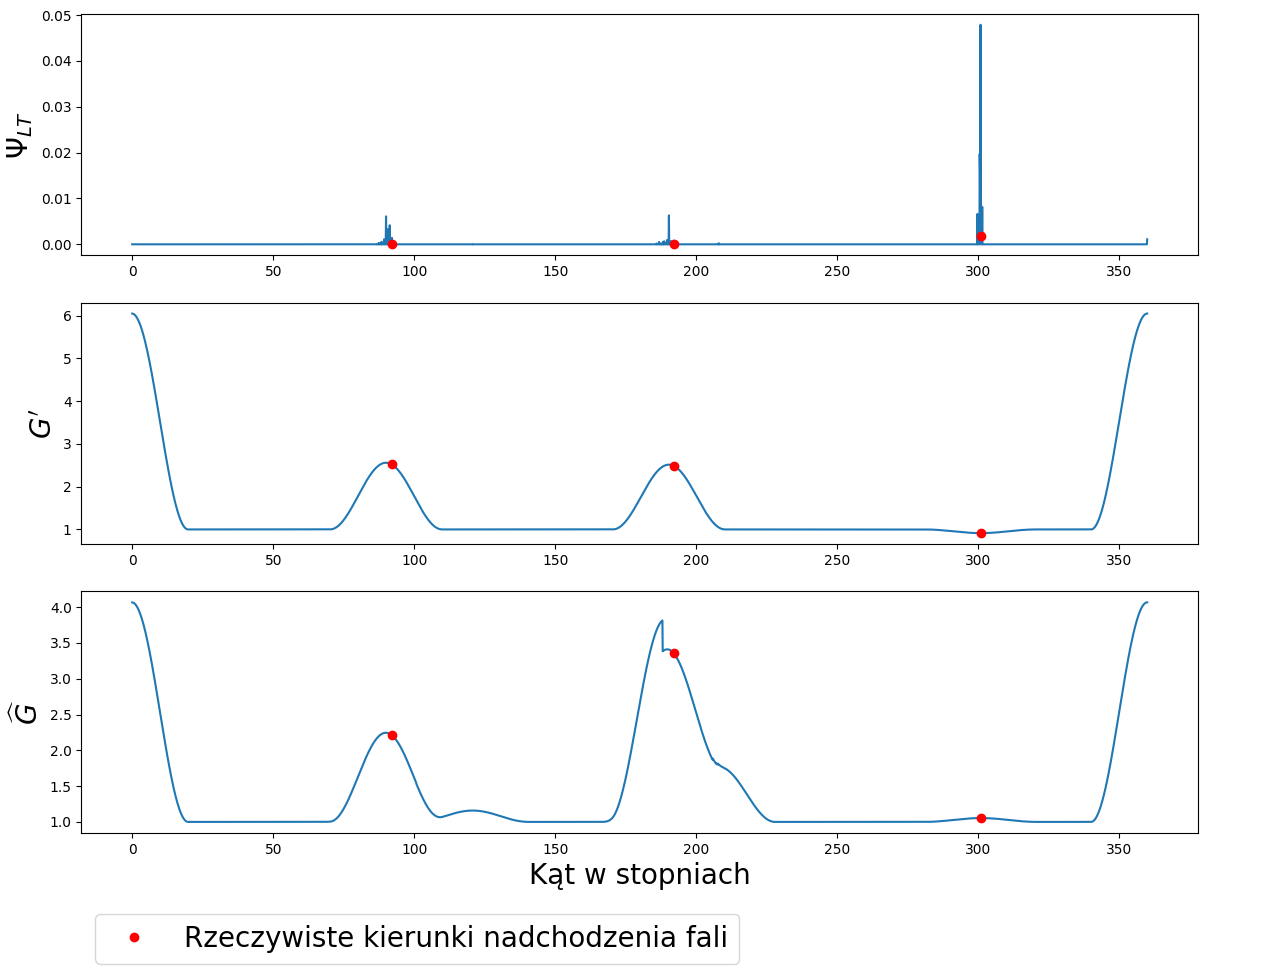
\includegraphics[width=\textwidth]{Images/moving_params_in_angle.png}
    \caption{Wybrane parametry jako funkcja kąta w pojedynczej ramce w przypadku ruchu jednego z nich}
    \label{fig:moving_params_in_angle}
\end{figure}

Zauważalną różnicą w stosunku do przypadku, w którym wszyscy użytkownicy byli statyczni jest różnica w położeniu pierwszej "górki" funkcji $G'$. Jest ona po prostu przesunięta. Stało się tak, ponieważ użytkownik zmienił już swoją pozycję w momencie obserwacji. Ruch nie powoduje pogorszenia się działania algorytmu.

\subsection{Odporność systemu na pogłos}

Ostatnim testowanym wariantem jest umieszczenie wszystkich trzech mówców w pokoju w celu ewualuacji działania algorytmu w modelu, w którym występuje duży pogłos. Otrzymane wyniki porównane zostaną z wynikami z wynikami eksperymentów bez pogłosu. Mówcy ponownie znajdują się na kątach $78^{\circ}$, $192^{\circ}$ i $301^{\circ}$. Wyniki znajdują się na wykresach \ref{fig:reverb}-\ref{fig:reverb_params_in_angle}.

\begin{figure}[h!]
    \centering
    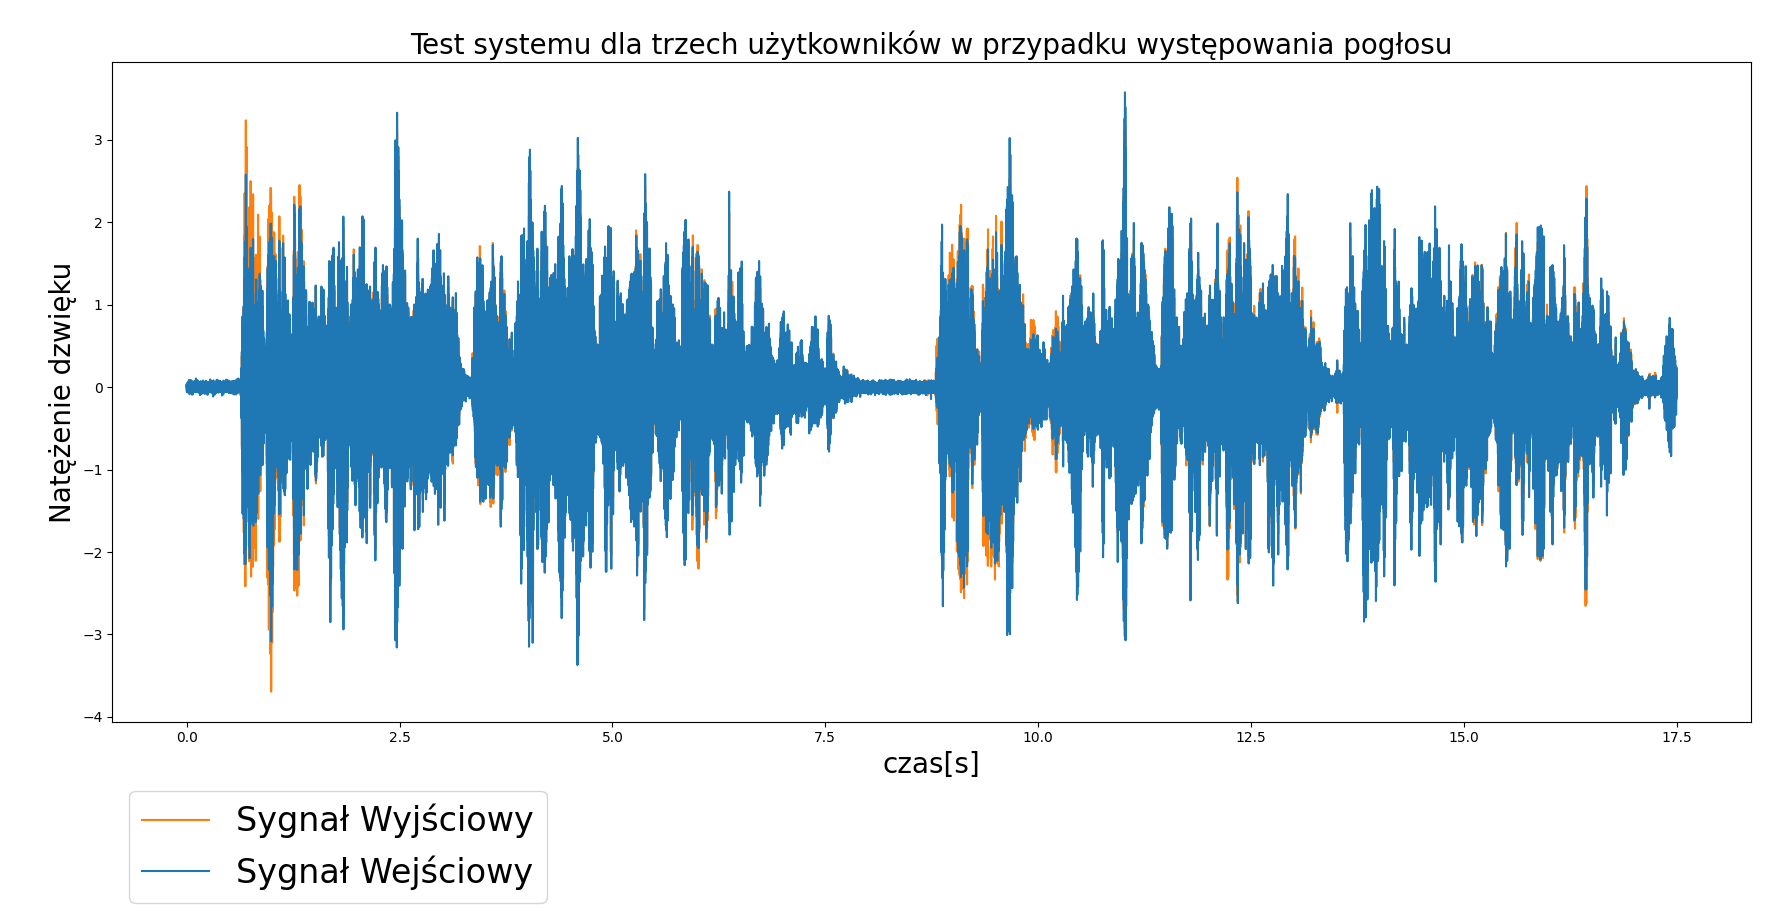
\includegraphics[width=\textwidth]{Images/reverb.png}
    \caption{Przebieg czasowy dla trzech mówców w przypadku występowania pogłosu}
    \label{fig:reverb}
\end{figure}

\begin{figure}[h!]
    \centering
    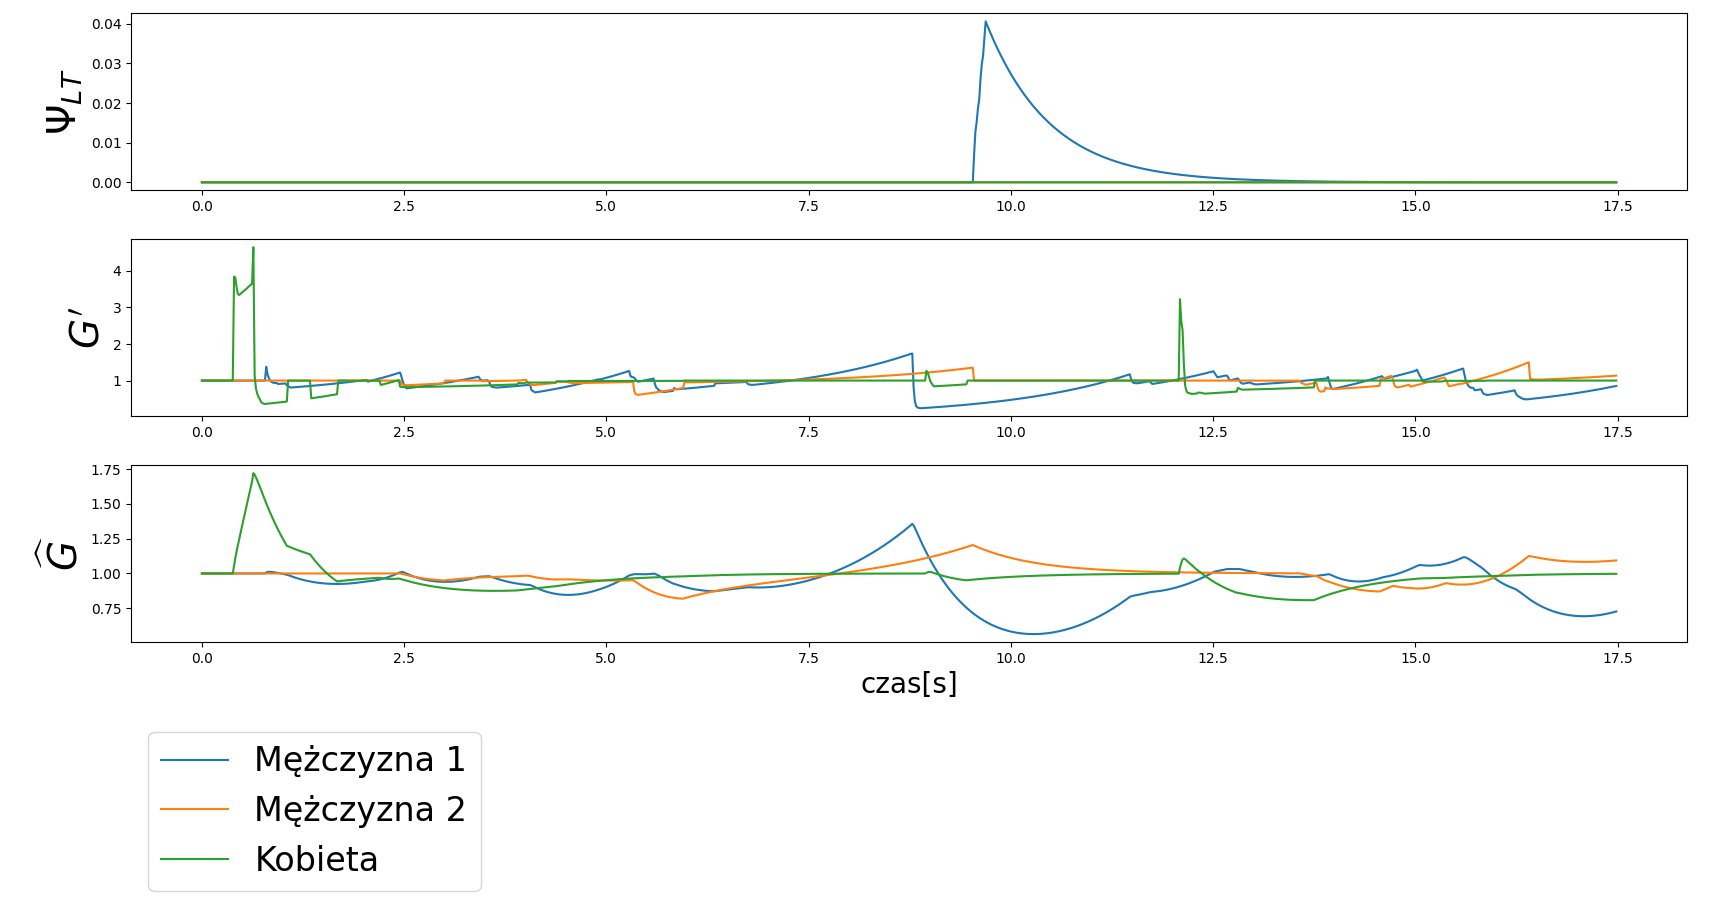
\includegraphics[width=\textwidth]{Images/reverb_params_in_time.png}
    \caption{Przebieg czasowy wybranych parametrów dla trzech mówców dla kierunków nadchodzenia fali w przypadku występowania pogłosu}
    \label{fig:reverb_params_in_time}
\end{figure}

\begin{figure}[h!]
    \centering
    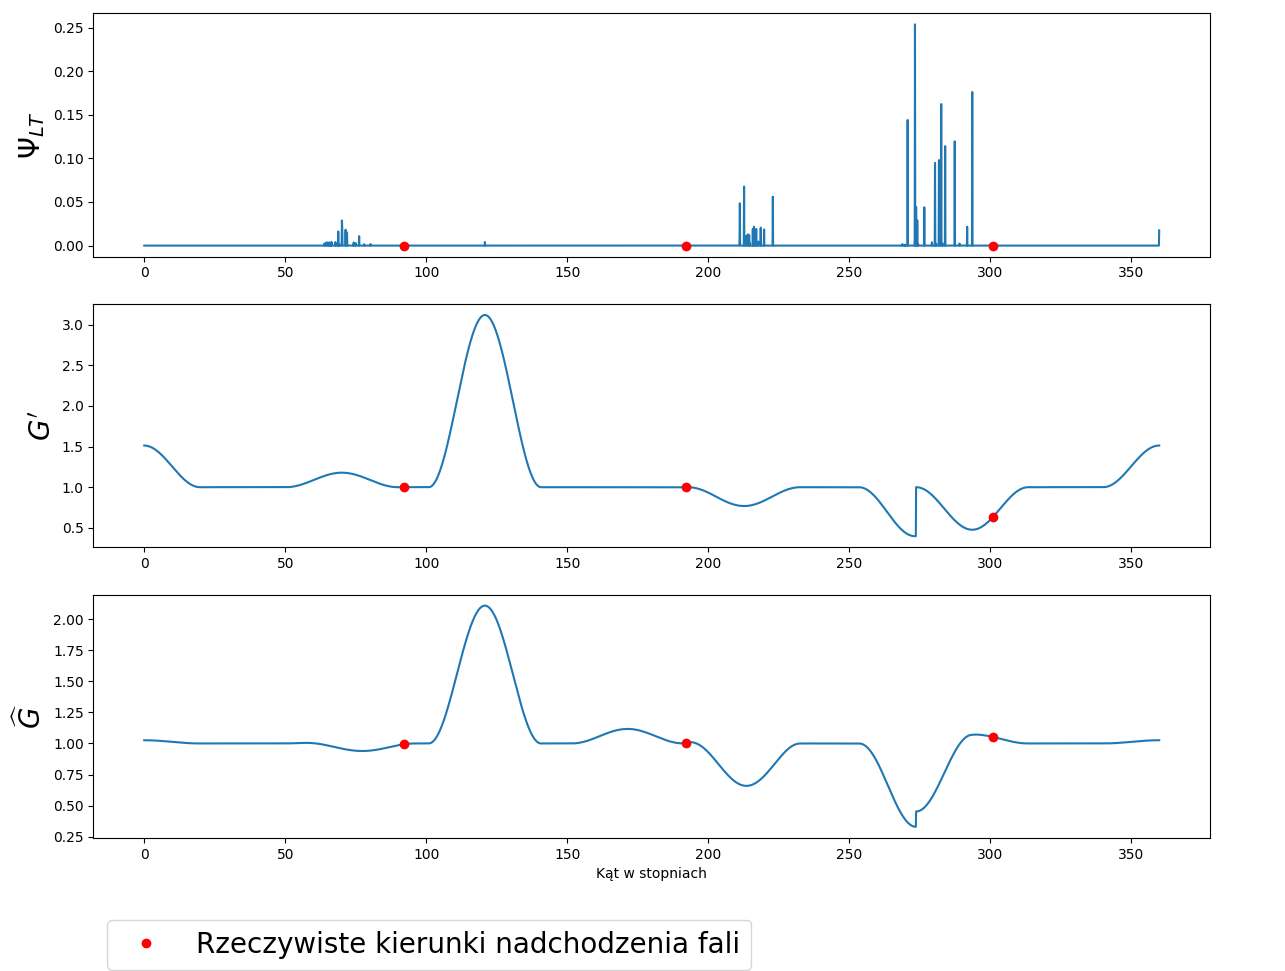
\includegraphics[width=\textwidth]{Images/reverb_params_in_angle.png}
    \caption{Wybrane parametry jako funkcja kąta w pojedynczej ramce w przypadku występowania pogłosu}
    \label{fig:reverb_params_in_angle}
\end{figure}

\noindent Na wykresie \ref{fig:reverb} obserwowany jest brak działania systemu AGC. Jak widać na wykresach następuje na tyle duży błąd estymacji kierunku nadchodzenia fali, że maksima funkcji $\widehat{G}$ są oddalone od kierunków nadchodzenia fali. Z tego powodu do równania \eqref{equation:constraint} brane są błędne kierunki. Oznacza to, że silny pogłos uniemożliwia praktyczne stosowanie algorytmu MUSIC do opisanego w tej pracy systemu.













